\section{Creating Weather Variables from Raw Data}

The weather variables used in the yield model estimation were created using raw data containing daily county level precipitation, vapor pressure deficit and maximum and minimum temperatures. The code used to create these variables for Iowa is shown, the equivalent procedure was completed in Ontario.

\subsection{Iowa - code used to create weather variables for yield model}

\begin{lstlisting}

setwd("C:/Users/Regan/Google Drive/Thesis Presentations and Proposal/Thesis")

N <- 99
T <- 58

iowa <- readRDS("Data needed to complete empirical work/Daily weather data/Iowa/weather_raw_daily.rds")
df <- iowa[order(iowa$county),]
df <- df[order(df$year),]

df <- df[df$days %in% c(1:65,67:366),]

attach(df)

hdd <- NULL
tot <- NULL
UPP <- 29
LOW <- 10

for (i in 1:nrow(df))
  {
  ifelse(i/20000==floor(i/20000),print(i),0)
  
  M <- (max[i]+min[i])/2
  W <- (max[i]-min[i])/2

  psi <- ifelse(max[i]>UPP,ifelse(min[i]<UPP,asin((UPP-M)/W),(-pi/2)),0)

  hdd[i] <- ifelse(max[i]>UPP,ifelse(min[i]<UPP,((M-UPP)*((pi/2)-psi)+W*cos(psi))/pi,M-UPP),0 )

  theta <- ifelse(max[i]>LOW,ifelse(min[i]<LOW,asin((LOW-M)/W),(-pi/2)),0)

  tot[i] <- ifelse(max[i]>LOW,ifelse(min[i]<LOW,((M-LOW)*((pi/2)-theta)+W*cos(theta))/pi,M-LOW),0)
}

gdd <- tot-hdd

fdd <- NULL
FREEZE <- -2
tot_cold <- NULL
COLD <- 2

for(i in 1:nrow(df))
{ifelse(i/20000==floor(i/20000),print(i),0)
  M <- (max[i]+min[i])/2
  W <- (max[i]-min[i])/2

  psi <- ifelse(min[i]<FREEZE,ifelse(max[i]>FREEZE,asin((FREEZE-M)/W),pi/2),0)
  
  fdd[i] <- ifelse(min[i]<FREEZE,ifelse(max[i]>FREEZE,((FREEZE-M)*(psi+(pi/2))+W*cos(psi))/pi,FREEZE-M),0)
  
  theta <- ifelse(min[i]<COLD,ifelse(max[i]>COLD,asin((COLD-M)/W),pi/2),0)
  
  tot_cold[i] <- ifelse(min[i]<COLD,ifelse(max[i]>COLD,((COLD-M)*(theta+pi/2)+W*cos(theta))/pi,COLD-M),0)}


cdd <- tot_cold-fdd

#calculating the gdd according to the agronomic formula in farenheit

max_farenheit <- (max*(9/5))+32
min_farenheit <- (min*(9/5))+32

max_gdd_ag <- (max_farenheit*as.numeric(max_farenheit<86))+(86*(max_farenheit>86))
max_gdd_ag <- (max_gdd_ag*as.numeric(max_gdd_ag>50))+(50*(max_gdd_ag<50))

min_gdd_ag <- (min_farenheit*as.numeric(min_farenheit>50))+(50*(min_farenheit<50))
min_gdd_ag <- (min_gdd_ag*as.numeric(min_gdd_ag<86))+(86*(min_gdd_ag>86))

gdd_ag <- ((max_gdd_ag+min_gdd_ag)/2-50)


#calculating the CHU according to method of OMAFRA

Ymax <- 3.33*(max-10)-0.084*((max-10)^2)
Ymax <- Ymax*(Ymax>0)

Ymin <- 1.8*(min-4.4)
Ymin <- Ymin*(Ymin>0)


CHU <- (Ymax+Ymin)/2

daily_weather_iowa <- data.frame(year,county,days,min,max,gdd,hdd,cdd,fdd,gdd_ag,pcp,vpd,CHU)

saveRDS(daily_weather_iowa,file="Data needed to complete empirical work/Daily weather data/Iowa/daily_weather_iowa")


\end{lstlisting}


\section{Estimating Planting Date}

\subsection{Iowa}

The planting date model was estimated using the calibrated planting date data for Iowa. This model was then used to create estimated planting dates for the years not included in the data set. The code for both the estimation of the planting model based on the calibrated planting data and its use to create estimated planting dates for all years included in the study is shown below. The results of the model estimation can be found in table 3.1 in the Methods section.

\subsubsection{Code for Creation of Planting Date Model and Planting Date Estimate in Iowa}



\begin{lstlisting}

setwd("C:/Users/Regan/Google Drive/Thesis Presentations and Proposal/Thesis")

weather <- readRDS("Data needed to complete empirical work/Daily weather data/Iowa/daily_weather_Iowa")

planting <- read.delim(file="Data needed to complete empirical work/Planting Date data/Iowa/county_planting_dates_iowa.txt",header=T,sep="\t")
silking <- read.delim(file="Data needed to complete empirical work/Planting Date data/Iowa/county_silking_dates_iowa.txt",header=T,sep="\t")

predict <- unique(planting\$year)
weather_predict <-  weather[weather\$year \%in\% predict,]

adjust <-seq(0,nrow(weather_predict)-365,365)

planting_row <- planting[,3]+adjust
silking_row <- silking[,3]+adjust

planting_day <- planting[,3]
silking_day <- silking[,3]

gdd_ag_accum <- NULL
for (i in 1:length(planting_row))
{gdd_ag_accum[i]<-sum(weather_predict$gdd_ag[planting_row[i]:silking_row[i]])}

median_gdd_accum <- summary(gdd_ag_accum)[3]

#####Modelling Planting Dates#####

###based on weather in the month of April###

April1 <- seq(91,nrow(weather_predict),365)
April30 <- seq(120,nrow(weather_predict),365)

mean_temp_daily <- (weather_predict$min+weather_predict$max)/2

mean_temp_April <- NULL
for(i in 1:length(April1))
{mean_temp_April[i]<-mean(mean_temp_daily[April1[i]:April30[i]])}

pcp_April <- NULL
for(i in 1:length(April1))
{pcp_April[i]<-mean(weather_predict$pcp[April1[i]:April30[i]])}

vpd_April <- NULL
for(i in 1:length(April1))
{vpd_April[i]<-mean(weather_predict$vpd[April1[i]:April30[i]])}

#we will add in the trend as it would be if all years were included#
#1974 - 20, 1986 - 32, 1988 - 34, 1991 - 37, 1993 - 39, 2012 - 58)

trend <- c(20:32,34:37,39:58)
Time <- matrix(0,99,length(trend))
for (i in 1:length(trend))
{Time[,i] <- rep(trend[i],99)}
trend <- as.vector(Time)

mod <- lm(planting_day ~ mean_temp_April+vpd_April+pcp_April+trend)

Beta_planting <- summary(mod)$coeff[,1]

#formatting table for latex using stargazer package#

install.packages("stargazer")
library(stargazer)
stargazer(mod, title="Planting Date Model Results", align=TRUE)

#####Creating the estimated planting dates from our model#####

###Creating the April weather data for all years in study###

April1 <- seq(91,nrow(weather),365)
April30 <- seq(120,nrow(weather),365)

mean_temp_daily <- (weather$min+weather$max)/2

mean_temp_April <- NULL
for(i in 1:length(April1))
{mean_temp_April[i]<-mean(mean_temp_daily[April1[i]:April30[i]])}

pcp_April <- NULL
for(i in 1:length(April1))
{pcp_April[i]<-mean(weather$pcp[April1[i]:April30[i]])}

vpd_April <- NULL
for(i in 1:length(April1))
{vpd_April[i]<-mean(weather$vpd[April1[i]:April30[i]])}

trend <- c(1:58)
Time <- matrix(0,99,length(trend))
for(i in 1:length(trend))
{Time[,i] <- rep(trend[i],99)}
trend <- as.vector(Time)

const <- rep(1,length(trend))

X <- cbind(const,mean_temp_April,vpd_April,pcp_April,trend)

planting_day_estimate <- X%*%Beta_planting

adjust <- seq(0,nrow(weather)-365,365)

planting_row_estimate <- planting_day_estimate+adjust

county <- rep(unique(weather$county),58)

year <- c(1955:2012)
Year <- matrix(0,99,length(year))
for(i in 1:length(year))
{Year[,i]<-rep(year[i],99)}
year <- as.vector(Year)

planting_day_estimate <- data.frame(cbind(year,county,planting_day_estimate))

###creating the estimated silking dates based on the planting dates###

#the silking dates will be the point at which the median gdd_ag accumulation occurs after planting date#

silking_row_estimate <- NULL

Aug30 <- seq(242,nrow(weather),365)
for(i in 1:length(planting_row_estimate))
{accum_gdd_ag <- 0
for(j in planting_row_estimate[i]:Aug30[i])
{accum_gdd_ag<- weather$gdd_ag[j]+accum_gdd_ag
if(accum_gdd_ag>=median_gdd_accum)
{silking_row_estimate[i] <- j
break}}
}

silking_day_estimate <- silking_row_estimate-adjust

silking_row_estimate <- data.frame(year,county,silking_row_estimate)
silking_day_estimate <- data.frame(year,county,silking_day_estimate)

#testing the level of error in the silking date estimates using known values

silk_test <- silking_day_estimate[silking_day_estimate$year %in% predict,]

silk_predict <- silk_test[,3]

mod <- lm(silking_day ~ 0+silk_predict)

#Residual standard error of 5.412 when using the predicted planting days to guess the known silking days#

###now we want to replace the known years with the values we have instead of keeping them as the predicted values###

new <- planting_day_estimate[planting_day_estimate$year %in% predict,]

rownumberknown <- row.names(new)

for (i in 1:length(rownumberknown))
{planting_day_estimate[rownumberknown[i],] <- planting[i,]}

for(i in 1:length(rownumberknown))
{silking_day_estimate[rownumberknown[i],] <- silking[i,]}

adjust <- seq(0,nrow(weather)-365,365)
planting_row_estimate <- planting_day_estimate[,3]+adjust
planting_row_estimate <- data.frame(year,county,planting_row_estimate)

silking_row_estimate <- silking_day_estimate[,3]+adjust
silking_row_estimate <- data.frame(year,county,silking_row_estimate)

saveRDS(planting_row_estimate,"Data needed to complete empirical work/Planting Date data/Iowa/planting_row_estimate")
saveRDS(silking_row_estimate,"Data needed to complete empirical work/Planting Date data/Iowa/silking_row_estimate")

\end{lstlisting}


\subsection{Ontario}

\subsubsection{Code for Creation of Planting Date Estimate in Ontario}

In Ontario there was no available planting date data which could be accessed. The method which has commonly been used by OMAFRA of taking the planting date to be the first day in the spring after which 3 days in a row have average temperatures of more than 12.8 degrees Celcius was used. \citep{OMAFRAhybrid}.

\begin{lstlisting}

setwd("C:/Users/Regan/Google Drive/Thesis Presentations and Proposal/Thesis")

weather <- readRDS("Data needed to complete empirical work/Daily weather data/Ontario/daily_weather_ontario")

counties <- c("brant","bruce","chatham-kent","dufferin","elgin","essex","grey","haldimand-norfolk",
		"halton","hamilton","hastings","huron","kawartha lakes","lambton","lanark",
		"leeds-grenville","lennox-addington","middlesex","niagara","northumberland",
		"ottawa","oxford","peel","perth","prescott-russell","prince edward","renfrew",
		"simcoe","stormont-dundas-glengarry","waterloo","wellington","york")


weather <- weather[weather$county %in% counties,]

attach(weather)

#calculating planting date as the day after 3 consecutive days with temp over 12.8 degrees celcius

April1 <-  seq(91,nrow(weather),365)
June1 <- seq(152,nrow(weather),365)
plant <- NULL
for(i in 1:length(April1))
{for(j in April1[i]:June1[i])
{if(((weather$max[j]+weather$min[j])/2)>=12.8 && ((weather$max[j+1]+weather$min[j+1])/2)>=12.8  && ((weather$max[j+2]+weather$min[j+2])/2)>=12.8)
{plant[i]<- (j+3)
break}
else{plant[i] <- (June1[i]+3)}}}

silk <- NULL

accum_gdd_ag <- 0
Aug30 <- seq(242,nrow(weather),365)
for(i in 1:length(plant))
{accum_gdd_ag <- 0
for(j in plant[i]:Aug30[i])
{accum_gdd_ag<- weather$gdd_ag[j]+accum_gdd_ag
if(accum_gdd_ag>=1400)
{silk[i] <- j
break}
else{silk[i] <- Aug30[i]}}}

year <- unique(year)
Year <- matrix(0,length(unique(county)),length(year))
for (i in 1:length(year))
{Year[,i]<-rep(year[i],length(unique(county)))}
year <- as.vector(Year)

county <- rep(unique(county),length(unique(year)))

planting_row_estimate <- plant
planting_row_estimate <- data.frame(year,county,planting_row_estimate)

silking_row_estimate <- silk
silking_row_estimate <- data.frame(year,county,silking_row_estimate)

saveRDS(planting_row_estimate,"Data needed to complete empirical work/Planting Date data/Ontario/planting_row_estimate")
saveRDS(silking_row_estimate,"Data needed to complete empirical work/Planting Date data/Ontario/silking_row_estimate")

\end{lstlisting}

\section{Model Testing}

As was discussed in the methods section various models with different combinations of variables and different ways of timing those variables were tested. To do this unique data sets which included variables corresponding to those required for each model were created. Each model was estimated using the corresponding created data set according to the procedure described in the methods section and the results were stored. Finally the most appropriate model was chosen based on the degree of model fit and the coefficient values. Below the various ways in which the variables were timed and the agronomic reasons for these timings are discussed.

\subsection{Agronomic Growth Stages and Growing Degree Days for Corn}

Growth stage dates are approximated by accumulated heat units beginning at the date of planting. Growing degree days (GDD) were used as the measure of accumulated heat units. Planting and silking data for the years that it was available in Iowa was used to test whether the agronomic estimates of the number of growing degree days which are accumulated from the planting date to the start of the silking date was accurate. Generally silking starts approximately when 1400 GDD have been accumulated since the planting date \citep{neild1987growing}. The median number of growing degree days which had accumulated between the calibrated planting and silking dates was 1389 and the mean was 1394, very similar to the 1400 generally assumed in theory. GDD accumulation from planting date estimates were used to time growth stages with silking stage assumed to start after 1389 GDD had accumulated. The table below shows the approximate growing degree day accumulations associated with the beginning of various corn growth stages.

\begin{table}[!htbp]
\caption{Corn Development and Growing Degree Days \citep{neild1987growing}}
\label{GDD_tab}
\begin{tabular}{lll}
\hline
Phase        & Development Stage                                                                                & GDD  \\
\hline
Vegetative   &                                                                                                  &      \\

             & Planted                                                                                          & 0    \\
             & Two leaves fully emerged                                                                         & 200  \\
             & Four eaves fully emerged                                                                         & 345  \\
             & Six leaves fully emerged (Growing point above soil) & 475  \\
             & Eight leaves fully emerged (Tassel beginning to develop)                                         & 610  \\
             & Ten leaves fully emerged                                                                         & 740  \\
             & Twelve leaves fully emerged (Ear formation)                                                      & 870  \\
             & Fourteen leaves fully emerged (Silks developing on ear)                                          & 1000 \\
             & Sixteen leaves fully emerged (Tip of tassel emerging)                                            & 1135 \\

Reproductive &                                                                                                  &      \\

             & Silks emerging/pollen shedding (Plant at full height)                                            & 1400 \\
             & Kernels in blister stage        & 1660 \\
             & Kernels in dough stage                                                                           & 1925 \\
             & Kernels denting                                                                                  & 2190 \\
Maturation   &                                                                                                  &      \\

             & Kernels dented                                                                                   & 2450 \\
             & Physiological maturity                                                                           & 2700\\
\hline
\end{tabular}
\end{table}


As the corn plant moves through these stages its input requirements change. As the number of leaves increase the plant is at an increased risk of damage from high temperatures and low precipitation levels \citep{neild1987growing}. As the tassel begins to emerge this sensitivity increases due to the possibility that pollen can be denatured from extreme heat or lack of water \citep{OMAFRA}. The silks emerge soon after this and are receptive to pollen. Environmental stress is very detrimental to yield at this point and stress due to lack of moisture in particular can damage the silks \citep{OMAFRA}. After pollination the grain filling period begins \citep{neild1987growing}. Precipitation after grain filling is complete is not as important for yield realization \citep{neild1987growing}. 

Detrimental effects from extreme heat reach a maximum during the silking and pollination period while cold temperature stress can be dangerous during early growth and emergence, or after pollination in the case of frost previous to denting \citep{OMAFRA}. Due to the distribution of temperature in North American climate it can be seen that extreme heat mostly occurs during the period at which it is most damaging. Cold temperatures are generally problematic at the beginning and end of the growing season which is the only time they are likely to occur. Because of this I did not alter the timing of any of the heat variables included in the various models when completing model testing and the heat variables are accumulations over the entire season. Therefore only the precipitation and vapour pressure deficit were subject to changes under different variable timing methods. Below I discuss the various timings that were considered.

\subsection{Variable Timing Profiles considered in Model Testing}

\subsubsection{Timing 0 - Mean of Variables over Growing Season}

Timing method 0 simply takes the averages of the precipitation and vapor pressure deficit variables over the entire growing season. The growing season is considered to begin at the estimated planting date and end at the estimated maturity date which is when 2700 growing degree days have accumulated after the planting date.

\subsubsection{Timing i - Accumulated Precipitation and Vapor Pressure Deficit over 3 stages of the Growing Season}

Timing i breaks up the growing season into 3 stages. The 3 stages correspond to the beginning of the season - planting to silking stage, the silking and pollination stage, and finally the end of the season - from pollination to maturity. The timing of the variables all have some days added to either side for buffering. The resulting variables are as follows:

$$\text{Precipitation for beginning of season stage: }PCP_b=sum(PCP(\text{planting:silking-5}))$$
$$\text{Precipitation for pollination stage: }PCP_pol=sum(PCP(\text{silking-4:silking+14}))$$
$$\text{Precipitation for end of season stage: }PCP_e=sum(PCP(\text{silking+15:maturity}))$$

Where $PCP$ refers to precipitation. The vapor pressure deficit variables are created in the same manner and using the same dates for timings. 

\subsubsection{Timing ii - Mean Precipitation and Vapor Pressure Deficit over 3 stages of the Growing Season}

Timing ii breaks up the stages of the growing season in the same way as timing i but takes the averages of the precipitation and vapor pressure deficit variables as opposed to their accumulated values over each period.

\subsubsection{Timing iii -  Accumulated Precipitation and Vapor Pressure Deficit for Each Month in the Growing Season}

Timing iii divides the growing season by month as opposed to by timed growth stages. The precipitation and vapor pressure deficit variables are the cumulative monthly totals from May to August when corn generally reaches maturity.

\subsubsection{Timing iv - Accumulated Precipitation and Vapor Pressure Deficit over 3 stages of the Growing Season}

Timing iv is similar to timing i in that it breaks up the growing season into 3 stages corresponding to a beginning of season stage, a pollination stage and an end of season stage. The difference with this timing is the amount of buffering applied to the variables. The timed variables are as shown below:

$$\text{Precipitation for beginning of season stage: }PCP_{b_i}=sum(PCP(\text{planting:silking-14}))$$
$$\text{Precipitation for pollination stage: }PCP_{pol_i}=sum(PCP(\text{silking-13:silking+14}))$$
$$\text{Precipitation for end of season stage: }PCP_{e_i}=sum(PCP(\text{silking+15:maturity}))$$

The vapor pressure deficit variables are created in the same manner and using the same dates for timings. 


\subsubsection{Timing v - Accumulated Precipitation and Vapor Pressure Deficit over 4 stages of the Growing Season}

Timing v splits the beginning of season precipitation variable into 2 parts. This is to consider the increasing demand for water which begins previous to the pollination and silking stage. The break point is set at the V10 stage which is marking approximately when 10 leaves have developed on the corn plant. The variables for this model are timed as shown below.

$$\text{Precipitation for beginning stage 1: }PCP_{b1_i}=sum(PCP(\text{planting:V10-10}))$$
$$\text{Precipitation for beginning stage 2: }PCP_{b1_i}=sum(PCP(\text{V10-9:silking-14}))$$
$$\text{Precipitation for pollination stage: }PCP_{pol_i}=sum(PCP(\text{silking-13:silking+14}))$$
$$\text{Precipitation for end of season stage: }PCP_{e_i}=sum(PCP(\text{silking+15:maturity}))$$

The vapor pressure deficit variables are created in the same manner and using the same dates for timings. 

\subsubsection{Timing vi - Mean of Variables over Growing Season}

Timing vi includes all of the variables in timing v but adds in an additional pre-season variable. This variable contains the accumulated pre-season precipitation and vapor pressure deficit respectively beginning in October of the previous year and ending at the time of planting. 

\subsection{Variable Groupings Considered in Model Testing}

In addition to the various methods of timing the precipitation and vapor pressure deficit variables we tested different combinations of the variables we were considering. These variables are average temperature over growing season (T), GDD, HDD, CDD, FDD, precipitation (P), and vapor pressure deficit (VPD). We tested models containing 7 different combinations of independent variables with each timing. The 7 different combinations are listed in the table below.

\begin{table}[!htbp]
\caption{Variable Grouping for Model Testing}
\label{var_groups_tab}
\begin{tabular}{l|lllllll}
\hline
                    & a & b & c & d & e & f & g \\
                    \hline
T                   & x & x &   &   &   &   &   \\
GDD                 &   &   & x & x & x & x & x \\
HDD                 &   &   &   & x & x & x & x \\
CDD                 &   &   &   &   & x &   & x \\
FDD                 &   &   &   &   &   & x & x \\
PCP                   & x & x & x & x & x & x & x \\
VPD                 &   & x & x & x & x & x & x\\
\hline
\end{tabular}
\end{table}

After the timed variables were created and grouped into data sets each timing and variable combination described was estimated as a linear model describing yields. 

\subsection{Code Used for Variable and Data set Creation for Model Testing}

The code used to create the variables and data sets for the first timing option (Timing 0) in Iowa is shown below. The generation and organization of the data for Ontario and for the other timings and combinations was very similar and is not included for the sake of space. 


\begin{lstlisting}

setwd("C:/Users/Regan/Google Drive/Thesis Presentations and Proposal/Thesis")

weather <- readRDS("Data needed to complete empirical work/Daily weather data/Iowa/daily_weather_Iowa")

#####Creating variables and data sets to test different models#####

###getting yield###

Yield <- readRDS("Data needed to complete empirical work/Yield Data/Iowa/Yield_Iowa")

yield <- Yield[,3]

year <- Yield[,1]

county <- Yield[,2]

###planting and silking date###

planting <- readRDS("Data needed to complete empirical work/Planting Date data/Iowa/planting_row_estimate")
planting <- planting[,3]

silking <- readRDS("Data needed to complete empirical work/Planting Date data/Iowa/silking_row_estimate")
silking <- silking[,3]

####0####
###a###

#mean temp and pcp over growing season#

May1 <- seq(121,nrow(weather),365)
Aug30 <- seq(242,nrow(weather),365)

mean_temp_daily <- (weather$min+weather$max)/2

mean_temp_season <- NULL
for(i in 1:length(May1))
{mean_temp_season[i] <- mean(mean_temp_daily[May1[i]:Aug30[i]])}

mean_pcp_season <- NULL
for(i in 1:length(May1))
{mean_pcp_season[i] <- mean(weather$pcp[May1[i]:Aug30[i]])}

trend <- c(1:58)
Trend <- matrix(0,99,length(trend))
for (i in 1:length(trend))
{Trend[,i] <- rep(trend[i],99)}
trend <- as.vector(Trend)


Data_a_0_iowa <- data.frame(year,county,yield,trend,mean_temp_season,mean_pcp_season)
\\
saveRDS(Data_a_0_iowa,"Data needed to complete empirical work/Data sets for model testing/Iowa/Data_a_0_iowa")

###b###

#mean temp, pcp and vpd over growing season#

mean_vpd_season <- NULL
for(i in 1:length(May1))
{mean_vpd_season[i] <- mean(weather$vpd[May1[i]:Aug30[i]])}

Data_b_0_iowa <- data.frame(year,county,yield,trend,mean_temp_season,mean_vpd_season,mean_pcp_season)
\\
saveRDS(Data_b_0_iowa,"Data needed to complete empirical work/Data sets for model testing/Iowa/Data_b_0_iowa")

###c###

#accumulated gdd mean pcp and vpd over growing season#

gdd_season <- NULL
for(i in 1:length(May1))
{gdd_season[i] <- sum(weather$gdd[May1[i]:Aug30[i]])}

Data_c_0_iowa <- data.frame(year,county,yield,trend,gdd_season,mean_vpd_season,mean_pcp_season)
\\
saveRDS(Data_c_0_iowa,"Data needed to complete empirical work/Data sets for model testing/Iowa/Data_c_0_iowa")

###d###

#gdd, hdd, mean pcp and vpd over growing season#

hdd_season <- NULL
for(i in 1:length(May1))
{hdd_season[i] <- sum(weather$hdd[May1[i]:Aug30[i]])}

Data_d_0_iowa <- data.frame(year,county,yield,trend,gdd_season,hdd_season,mean_vpd_season,mean_pcp_season)
\\
saveRDS(Data_d_0_iowa,"Data needed to complete empirical work/Data sets for model testing/Iowa/Data_d_0_iowa")

###e###

#d plus cdd#

cdd_season <- NULL
for(i in 1:length(May1))
{cdd_season[i] <- sum(weather$cdd[May1[i]:Aug30[i]])}

Data_e_0_iowa <- data.frame(year,county,yield,trend,gdd_season,hdd_season,cdd_season,mean_vpd_season,mean_pcp_season)
\\
saveRDS(Data_e_0_iowa,"Data needed to complete empirical work/Data sets for model testing/Iowa/Data_e_0_iowa")

###f###

#e with fdd subbed for cdd#

fdd_season <- NULL
for(i in 1:length(May1))
{fdd_season[i] <- sum(weather$fdd[May1[i]:Aug30[i]])}

Data_f_0_iowa <- data.frame(year,county,yield,trend,gdd_season,hdd_season,fdd_season,mean_vpd_season,mean_pcp_season)
\\
saveRDS(Data_f_0_iowa,"Data needed to complete empirical work/Data sets for model testing/Iowa/Data_f_0_iowa")

###g###

#f with cdd as well#

Data_g_0_iowa <- data.frame(year,county,yield,trend,gdd_season,hdd_season,cdd_season,fdd_season,mean_vpd_season,mean_pcp_season)
\\
saveRDS(Data_g_0_iowa,"Data needed to complete empirical work/Data sets for model testing/Iowa/Data_g_0_iowa")



\end{lstlisting}



\subsection{Results from Model Testing}

In the methods section the spatial nature of the data was discussed. The spatial correlation parameter is first estimated by maximizing the likelihood equation as described in the methods section. Then the model is reconfigured using this $\rho$ value to give $X_{new}=AX$ and $Y_{new}=AY$. The regression of $Y_{new}$ on $X_{new}$ can then be estimated by OLS. Therefore the dependent variable in the results below is $Y_{new}$ and the independent variables are the columns of $X_{new}$, however they are referred to by their variable names as they would have been in $X$. Regional dummy variables were included in each Iowa model for the 9 regions in the state and county dummy variables were included in each Ontario model for all 32 counties in the data set. In the results tables below the estimated coefficients for all of the dummy variables both in Iowa and Ontario have been removed for the sake of brevity given that they are not the variables of interest.

\subsubsection{Iowa}


 
\begin{table}[H]
    \centering
    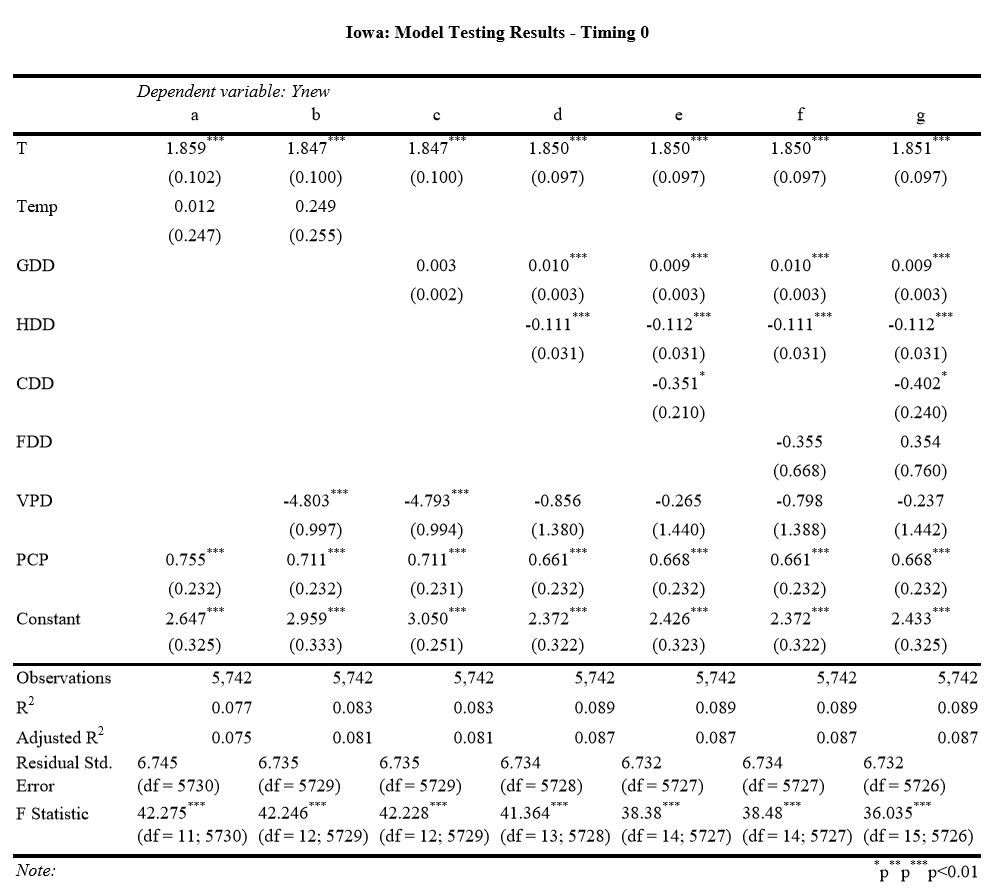
\includegraphics[width=1.0\textwidth]{IA_a_0.png}
    \caption{Iowa: Model Testing Results - Timing 0}
    \label{fig:my_label}
\end{table}

 
\begin{table}[H]
    \centering
    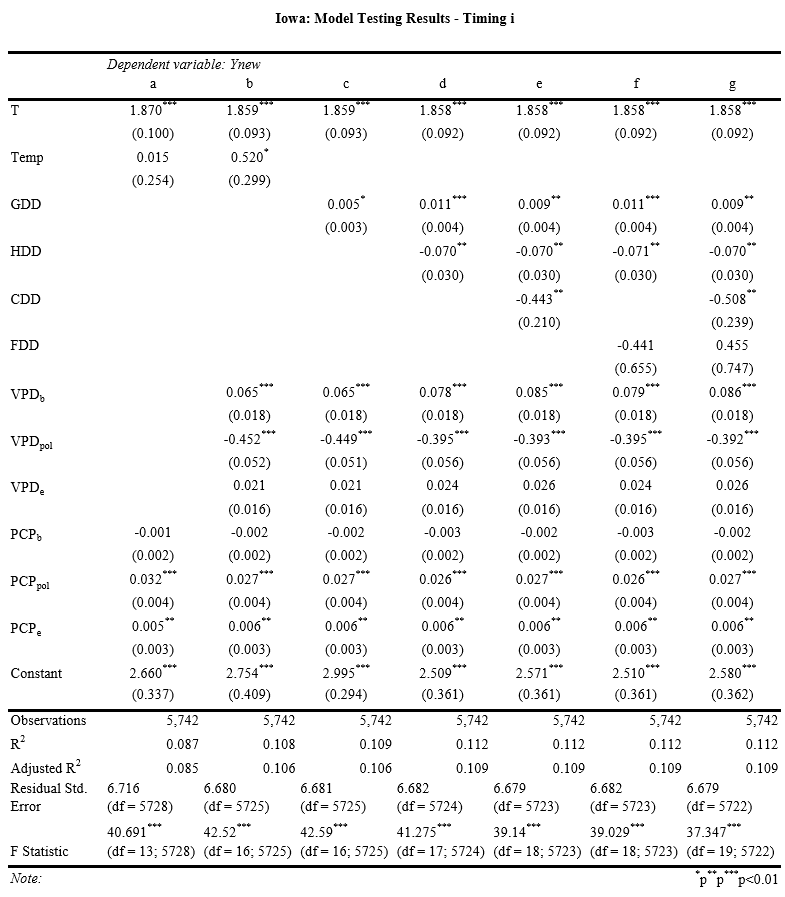
\includegraphics[width=1.0\textwidth]{IA_a_i.png}
    \caption{Iowa: Model Testing Results - Timing i}
    \label{fig:my_label}
\end{table}

 
\begin{table}[H]
    \centering
    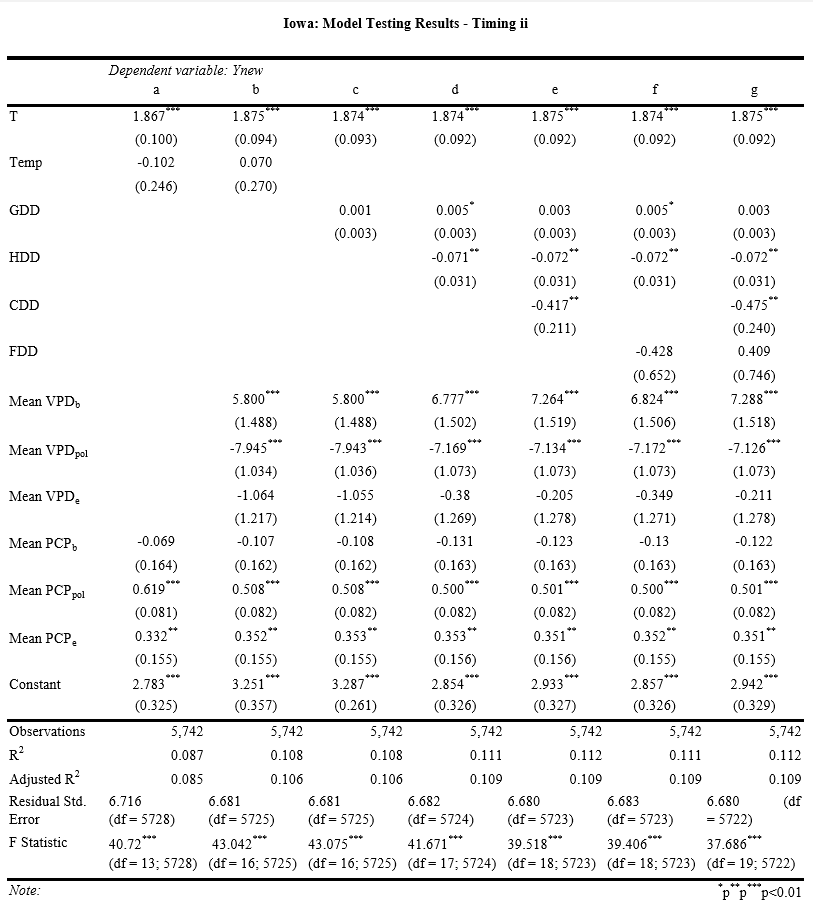
\includegraphics[width=1.0\textwidth]{IA_a_ii.png}
    \caption{Iowa: Model Testing Results - Timing ii}
    \label{fig:my_label}
\end{table}

 
\begin{table}[H]
    \centering
    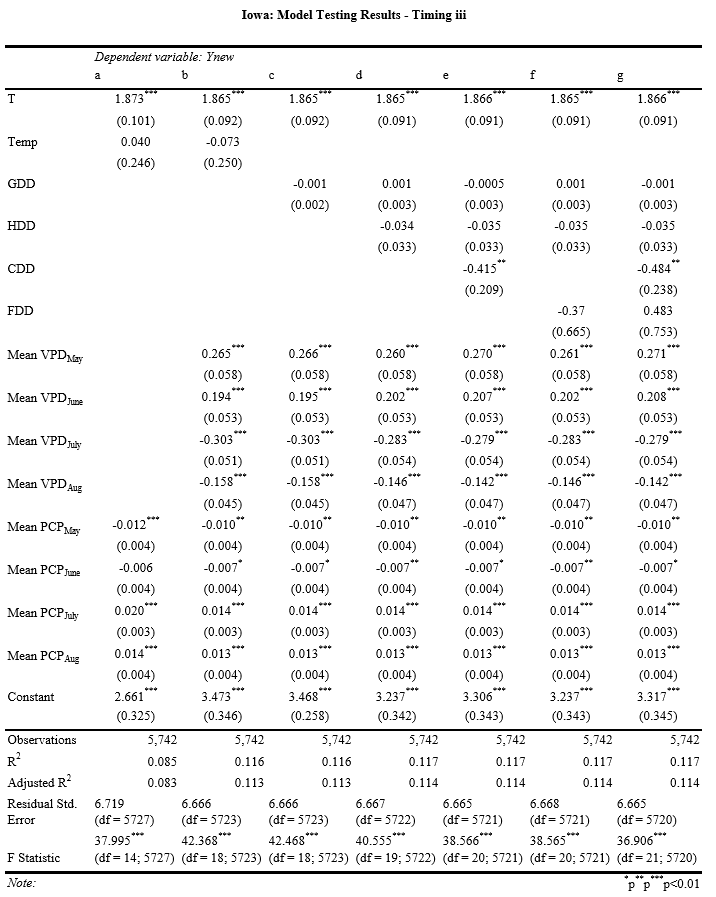
\includegraphics[width=1.0\textwidth]{IA_a_iii.png}
    \caption{Iowa: Model Testing Results - Timing iii}
    \label{fig:my_label}
\end{table}

 
\begin{table}[H]
    \centering
    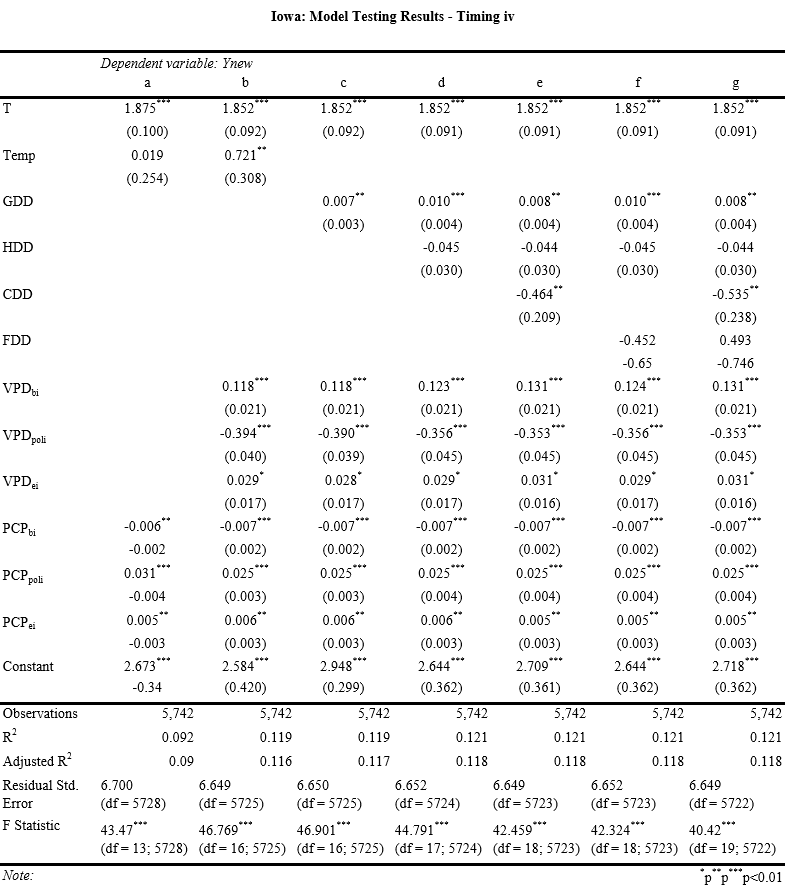
\includegraphics[width=1.0\textwidth]{IA_a_iv.png}
    \caption{Iowa: Model Testing Results - Timing iv}
    \label{fig:my_label}
\end{table}

 
\begin{table}[H]
    \centering
    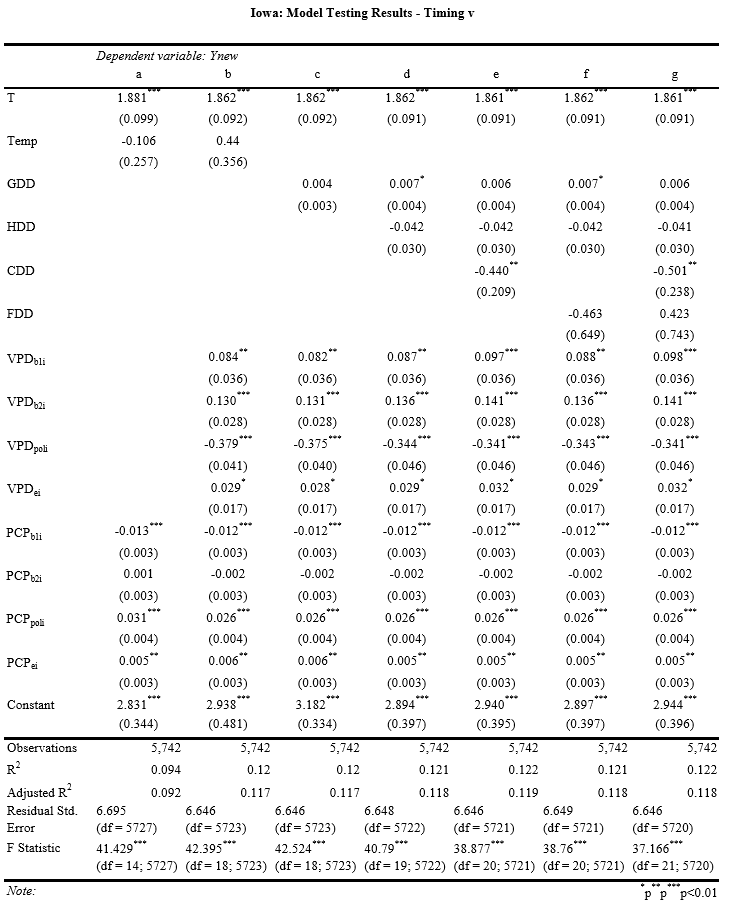
\includegraphics[width=1.0\textwidth]{IA_a_v.png}
    \caption{Iowa: Model Testing Results - Timing v}
    \label{fig:my_label}
\end{table}

 
\begin{table}[H]
    \centering
    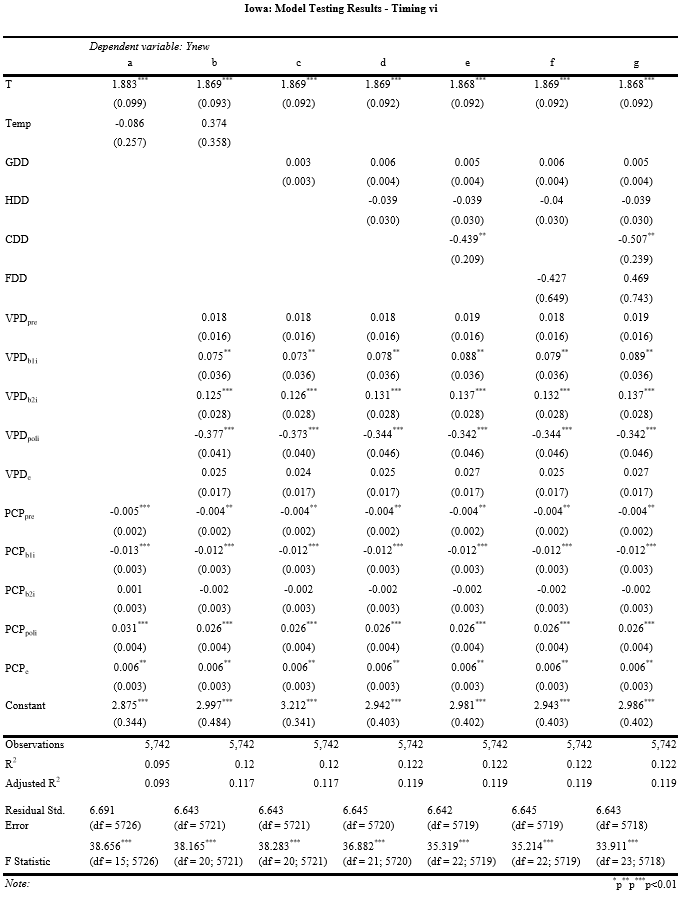
\includegraphics[width=1.0\textwidth]{IA_a_vi.png}
    \caption{Iowa: Model Testing Results - Timing vi}
    \label{fig:my_label}
\end{table}



\subsubsection{Ontario}

 
\begin{table}[H]
    \centering
    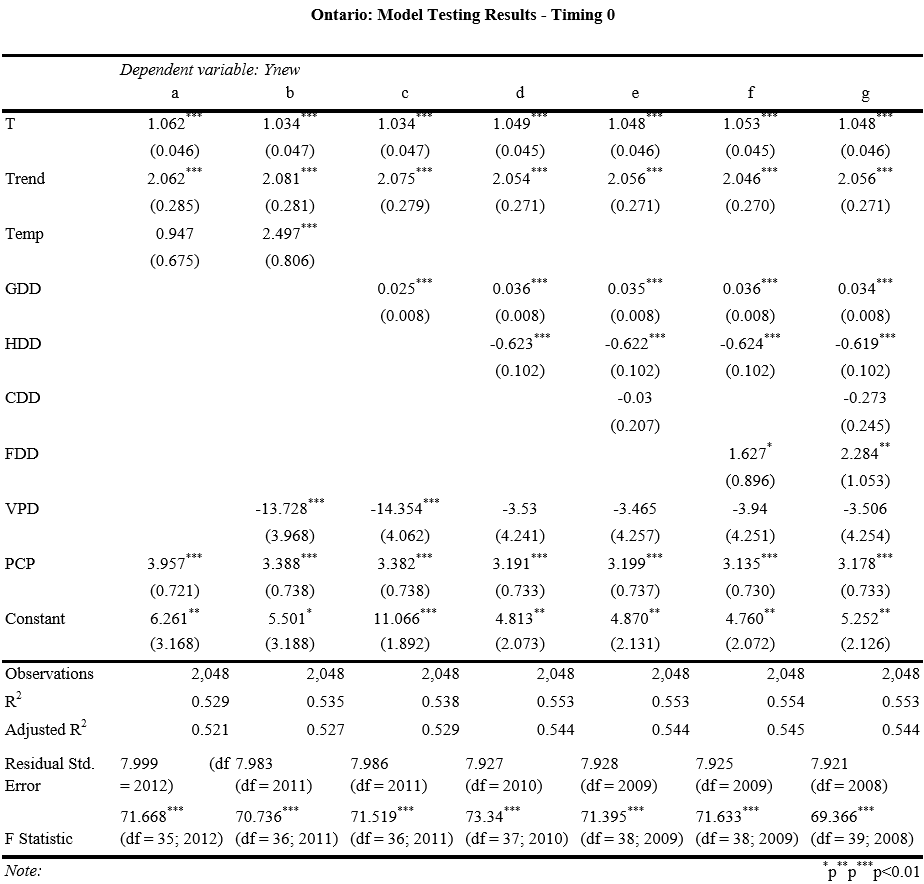
\includegraphics[width=1.0\textwidth]{ON_a_0.png}
    \caption{Ontario: Model Testing Results - Timing 0}
    \label{fig:my_label}
\end{table}

\begin{table}[H]
    \centering
    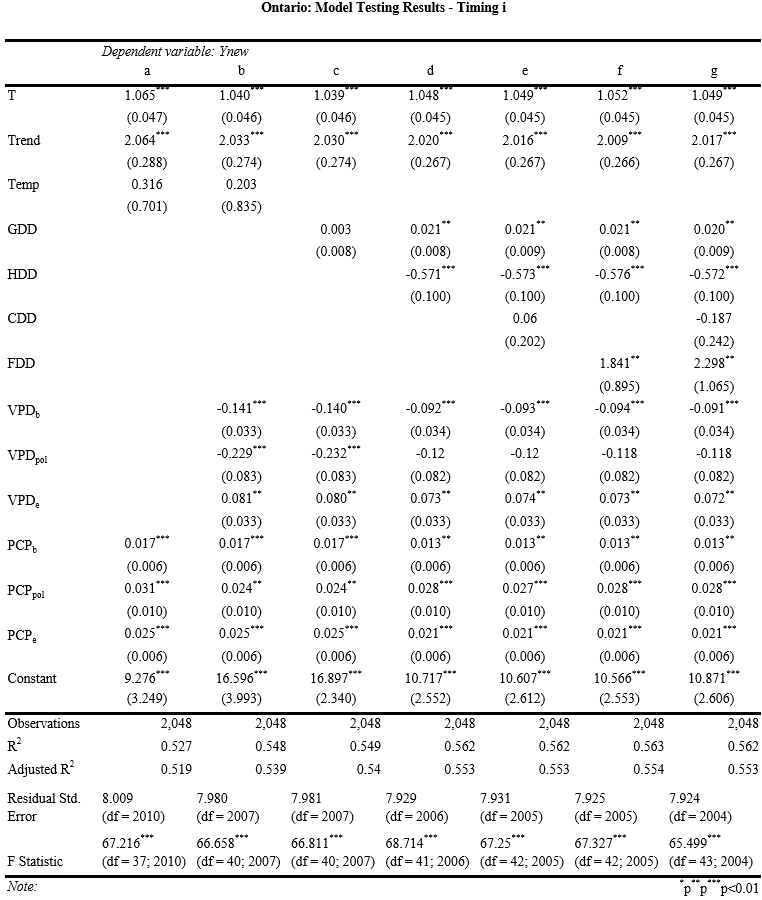
\includegraphics[width=1.0\textwidth]{ON_a_i.png}
    \caption{Ontario: Model Testing Results - Timing i}
    \label{fig:my_label}
\end{table}

\begin{table}[H]
    \centering
    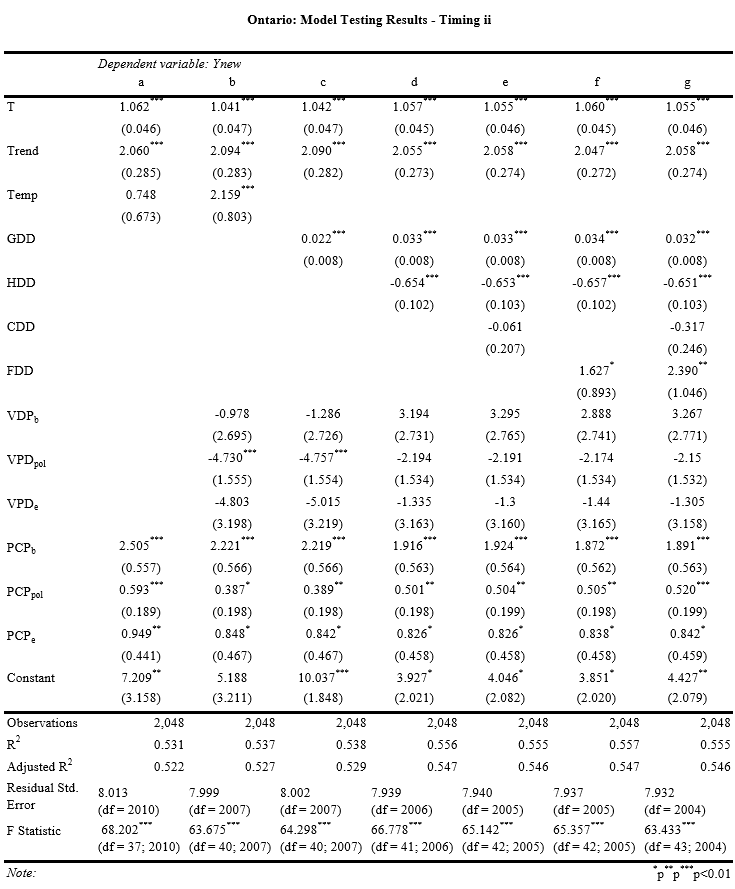
\includegraphics[width=1.0\textwidth]{ON_a_ii.png}
    \caption{Ontario: Model Testing Results - Timing ii}
    \label{fig:my_label}
\end{table}

\begin{table}[H]
    \centering
    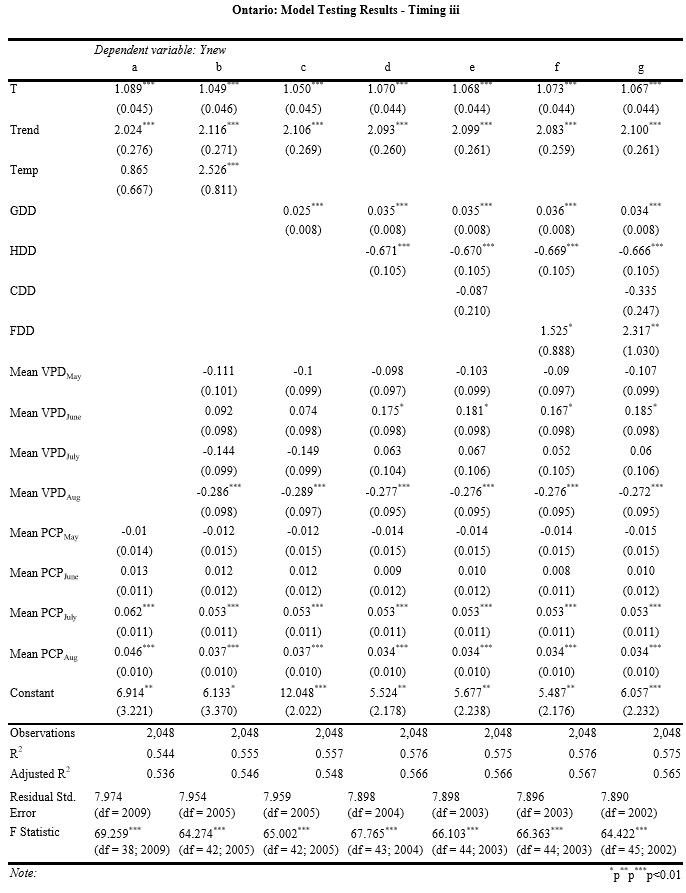
\includegraphics[width=1.0\textwidth]{ON_a_iii.png}
    \caption{Ontario: Model Testing Results - Timing iii}
    \label{fig:my_label}
\end{table}

\begin{table}[H]
    \centering
    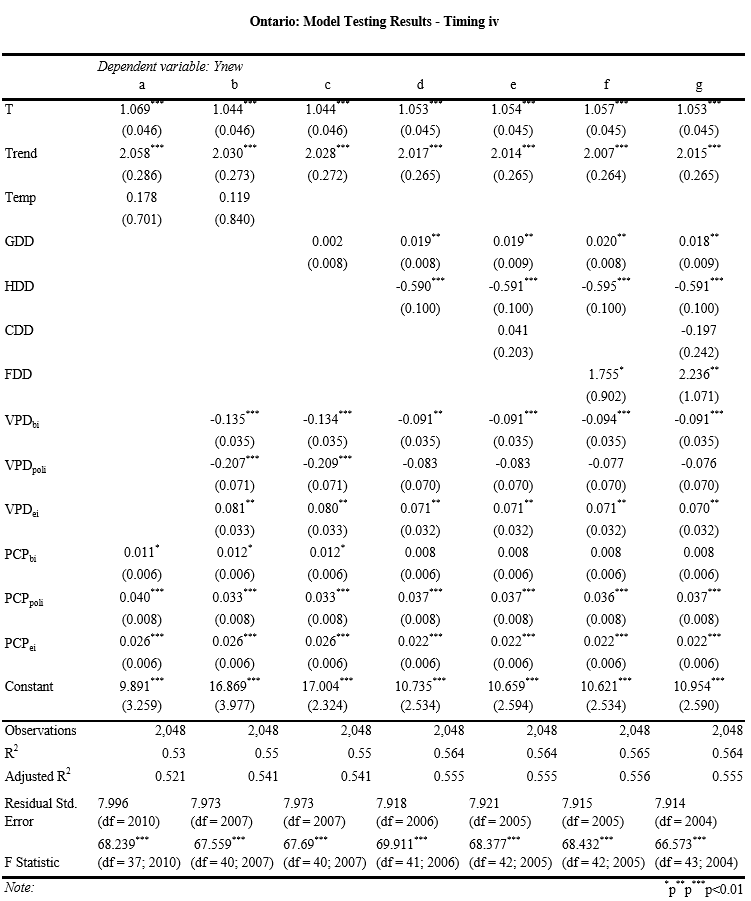
\includegraphics[width=1.0\textwidth]{ON_a_iv.png}
    \caption{Ontario: Model Testing Results - Timing iv}
    \label{fig:my_label}
\end{table}

\begin{table}[H]
    \centering
    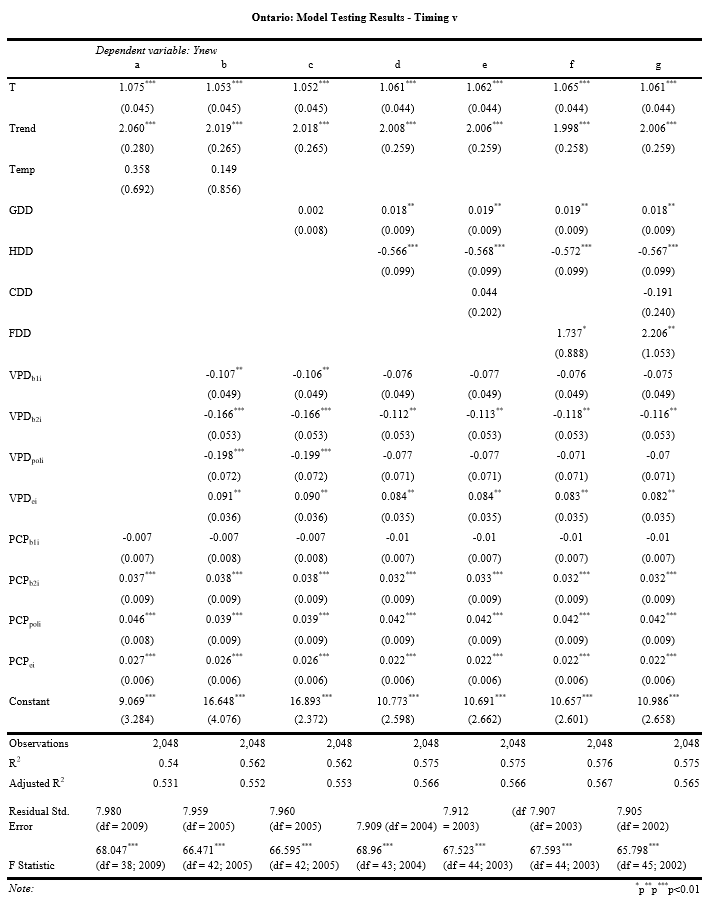
\includegraphics[width=1.0\textwidth]{ON_a_v.png}
    \caption{Ontario: Model Testing Results - Timing v}
    \label{fig:my_label}
\end{table}

\begin{table}[H]
    \centering
    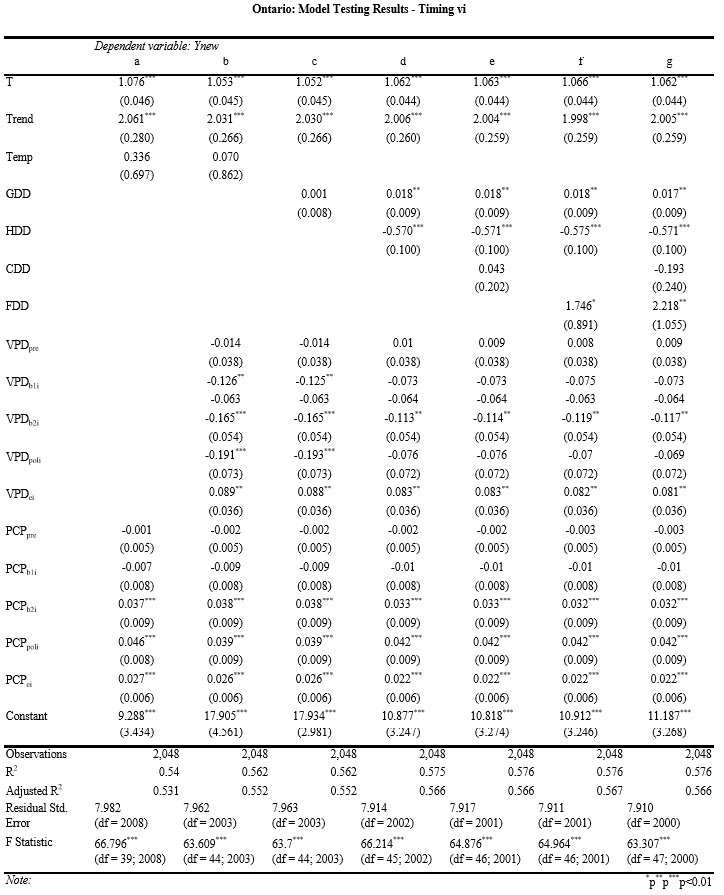
\includegraphics[width=1.0\textwidth]{ON_a_vi.png}
    \caption{Ontario: Model Testing Results - Timing vi}
    \label{fig:my_label}
\end{table}

\begin{table}[H]
   
    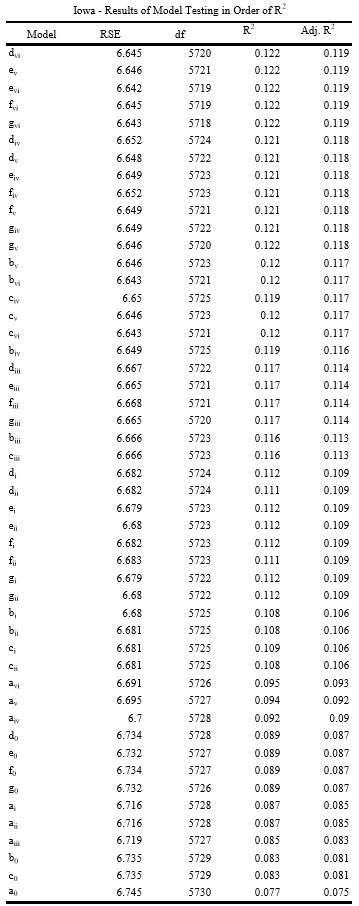
\includegraphics[width=.55\textwidth]{Iowa_r2.png}
    \caption{Iowa - Results of Model Testing in Order of R$^2$}
    \label{fig:my_label}
\end{table}

\begin{table}[H]
   
    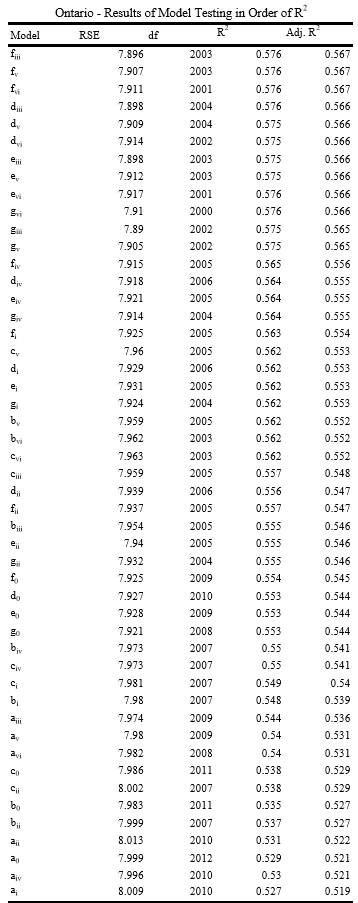
\includegraphics[width=.55\textwidth]{Ontario_r2.png}
    \caption{Ontario - Results of Model Testing in Order of R$^2$}
    \label{fig:my_label}
\end{table}


Model $div$ was chosen for Iowa. This model was selected as it was the most parsimonious model with the highest adjusted $R^2$. In Ontario the 3 models which tied for the highest adjusted $R^2$ had large positive coefficients on the FDD terms which were about 2.5 to 3 times the magnitude of the HDD coeficients from the same models. FDD represents temperatures below -2 degrees celcius which can damage corn yields when they occur both at the beginning and the end of the season \citep{OMAFRA}. These results were not logical and therefore the simpler $diii$ model was chosen for Ontario as it also had a high adjusted $R^2$.



\subsection{Code from Model Testing}

The following code was used to test each of the models considered. The data set df was set at the top and the model was evaluated given the particular combination of variables in that particular data set.

\subsubsection{Iowa}

\begin{lstlisting}


setwd("C:/Users/Regan/Google Drive/Thesis Presentations and Proposal/Thesis")

N <- 99
T <- 58

Dummy <- read.delim("Data needed to complete empirical work/Data sets for model testing/Iowa/county_region_matrix.txt")

Dummy <- Dummy[,2:9]

Dummy <- apply(Dummy,2,as.numeric)

Dummy <- matrix( rep( t(Dummy) , T ) , ncol = ncol(Dummy) , byrow = TRUE )

NW <- Dummy[,1]
NC <- Dummy[,2]
NE <- Dummy[,3]
WC <- Dummy[,4]
C <- Dummy[,5]
EC <- Dummy[,6]
SW <- Dummy[,7]
SC <- Dummy[,8]
#SE is the point of comparison#

df <- readRDS("Data needed to complete empirical work/Data sets for model testing/Iowa/Data_a_0_iowa")

Y <- df[,3]

const <- rep(1,N*T)
X <- as.matrix(cbind(const,df[,4:ncol(df)],NW,NC,NE,WC,C,EC,SW,SC))

W <- read.delim("Data needed to complete empirical work/Data sets for model testing/Iowa/Iowa_W_norm.txt", header=F)
W <- as.matrix(W)

K <- kronecker(diag(T),W)

eig <- eigen(W, symmetric = FALSE, only.values = TRUE)
lambda <- eig$values

rhomin <- (1/min(lambda))
rhomax <- (1/max(lambda))

p_bound <- seq(rhomin,rhomax,.1)

log_L <- function(p)
{A <- (diag(N*T)-p*K)
log_det_I_pW <- log(1-p*lambda)
log_detA <- T*sum(log_det_I_pW)
Beta <- solve(t(A%*%X)%*%(A%*%X))%*%t(A%*%X)%*%(A%*%Y)
U <- Y-X%*%Beta
sigma_sq <- (1/N*T)*(t(U)%*%t(A)%*%A%*%U)
log_L <- (-(N*T)/2)*log(2*pi*sigma_sq)+log_detA-(1/(2*sigma_sq))*t(U)%*%t(A)%*%A%*%U
return(-log_L)}

p_opt <- optim(mean(p_bound),(log_L),method="Brent",lower=rhomin, upper=rhomax)$par

A <- (diag(N*T)-p_opt*K)
Ynew <- A%*%Y

X1 <- as.matrix(cbind(df[,4:ncol(df)],NW,NC,NE,WC,C,EC,SW,SC))

Xnew <- A%*%X1

mod <- lm(Ynew~Xnew)


a_vi <- mod
b_vi <- mod
c_vi <- mod
d_vi <- mod
e_vi <- mod
f_vi <- mod
g_vi <- mod


install.packages("sandwich")
library(sandwich)

# Adjust standard errors
cov_a_vi         <- vcovHC(a_vi, type = "HC3")
robust_a_vi    <- sqrt(diag(cov_a_vi))

cov_b_vi         <- vcovHC(b_vi, type = "HC3")
robust_b_vi    <- sqrt(diag(cov_b_vi))

cov_c_vi         <- vcovHC(c_vi, type = "HC3")
robust_c_vi    <- sqrt(diag(cov_c_vi))

cov_d_vi         <- vcovHC(d_vi, type = "HC3")
robust_d_vi    <- sqrt(diag(cov_d_vi))

cov_e_vi         <- vcovHC(e_vi, type = "HC3")
robust_e_vi    <- sqrt(diag(cov_e_vi))

cov_f_vi         <- vcovHC(f_vi, type = "HC3")
robust_f_vi    <- sqrt(diag(cov_f_vi))

cov_g_vi         <- vcovHC(g_vi, type = "HC3")
robust_g_vi    <- sqrt(diag(cov_g_vi))


install.packages("lmtest")
library(lmtest)

wald_results_a_vi <- waldtest(a_vi, vcov = cov_a_vi)
wald_results_b_vi <- waldtest(b_vi, vcov = cov_b_vi)
wald_results_c_vi <- waldtest(c_vi, vcov = cov_c_vi)
wald_results_d_vi <- waldtest(d_vi, vcov = cov_d_vi)
wald_results_e_vi <- waldtest(e_vi, vcov = cov_e_vi)
wald_results_f_vi <- waldtest(f_vi, vcov = cov_f_vi)
wald_results_g_vi <- waldtest(g_vi, vcov = cov_g_vi)



install.packages("stargazer")
library(stargazer)

stargazer(a_vi,b_vi,c_vi,d_vi,e_vi,f_vi,g_vi,type="html",title = "Iowa: Model Testing Results - Timing vi",column.labels = c("a_vi","b_vi", "c_vi", "d_vi", "e_vi$", "f_vi", "g_vi" ),se=list(robust_a_vi,robust_b_vi,robust_c_vi,robust_d_vi,robust_e_vi,robust_f_vi,robust_g_vi), align=TRUE,out = "Result tables/Iowa_model_a_vi_results.html")


\end{lstlisting}

\subsubsection{Ontario}

\begin{lstlisting}
######Model Testing######

#####Regional Dummy#####

setwd("C:/Users/Regan/Google Drive/Thesis Presentations and Proposal/Thesis")

N <- 32
T <- 64

Dummy <- diag(N)
Dummy <- matrix( rep( t( Dummy) , T ) , ncol = ncol(Dummy) , byrow = TRUE )


###a_0###

df <- readRDS("Data needed to complete empirical work/Data sets for model testing/Ontario/Data_a_0_ont")

Y <- df[,3]

const <- rep(1,N*T)
X <- as.matrix(cbind(const,df[,4:ncol(df)],Dummy[,1:31]))

W <- read.delim("Code/Ontario/W_ONT_norm.txt",header=F)
W <- as.matrix(W)

K <- kronecker(diag(T),W)

eig <- eigen(W, symmetric = FALSE, only.values = TRUE)
lambda <- eig$values

rhomin <- (1/min(lambda))
rhomax <- (1/max(lambda))

p_bound <- seq(rhomin,rhomax,.1)

log_L <- function(p)
{A <- (diag(N*T)-p*K)
log_det_I_pW <- log(1-p*lambda)
log_detA <- T*sum(log_det_I_pW)
Beta <- solve(t(A%*%X)%*%(A%*%X))%*%t(A%*%X)%*%(A%*%Y)
U <- Y-X%*%Beta
sigma_sq <- (1/N*T)*(t(U)%*%t(A)%*%A%*%U)
log_L <- (-(N*T)/2)*log(2*pi*sigma_sq)+log_detA-(1/(2*sigma_sq))*t(U)%*%t(A)%*%A%*%U
return(-log_L)}



p_opt <- optim(mean(p_bound),(log_L),method="Brent",lower=rhomin, upper=rhomax)$par

A <- (diag(N*T)-p_opt*K)
Ynew <- A%*%Y

X1 <- as.matrix(cbind(df[,4:ncol(df)],Dummy[,1:31]))

Xnew <- A%*%X1

mod <- lm(Ynew~Xnew)

a_vi <- mod
b_vi <- mod
c_vi <- mod
d_vi <- mod
e_vi <- mod
f_vi <- mod
g_vi <- mod


install.packages("sandwich")
library(sandwich)

# Adjust standard errors
cov_a_vi         <- vcovHC(a_vi, type = "HC3")
robust_a_vi    <- sqrt(diag(cov_a_vi))

cov_b_vi         <- vcovHC(b_vi, type = "HC3")
robust_b_vi    <- sqrt(diag(cov_b_vi))

cov_c_vi         <- vcovHC(c_vi, type = "HC3")
robust_c_vi    <- sqrt(diag(cov_c_vi))

cov_d_vi         <- vcovHC(d_vi, type = "HC3")
robust_d_vi    <- sqrt(diag(cov_d_vi))

cov_e_vi         <- vcovHC(e_vi, type = "HC3")
robust_e_vi    <- sqrt(diag(cov_e_vi))

cov_f_vi         <- vcovHC(f_vi, type = "HC3")
robust_f_vi    <- sqrt(diag(cov_f_vi))

cov_g_vi         <- vcovHC(g_vi, type = "HC3")
robust_g_vi    <- sqrt(diag(cov_g_vi))


install.packages("lmtest")
library(lmtest)

wald_results_a_vi <- waldtest(a_vi, vcov = cov_a_vi)
wald_results_b_vi <- waldtest(b_vi, vcov = cov_b_vi)
wald_results_c_vi <- waldtest(c_vi, vcov = cov_c_vi)
wald_results_d_vi <- waldtest(d_vi, vcov = cov_d_vi)
wald_results_e_vi <- waldtest(e_vi, vcov = cov_e_vi)
wald_results_f_vi <- waldtest(f_vi, vcov = cov_f_vi)
wald_results_g_vi <- waldtest(g_vi, vcov = cov_g_vi)



install.packages("stargazer")
library(stargazer)


stargazer(a_vi,b_vi,c_vi,d_vi,e_vi,f_vi,g_vi,type="html",title = "Ontario: Model Testing Results - Timing vi",column.labels = c("a_vi","b_vi", "c_vi", "d_vi", "e_vi$", "f_vi", "g_vi" ),se=list(robust_a_vi,robust_b_vi,robust_c_vi,robust_d_vi,robust_e_vi,robust_f_vi,robust_g_vi), align=TRUE,out = "Result tables/Ontario_model_a_vi_results.html")



\end{lstlisting}



\section{Solving for Optimal Threshold Values}

In the methods section the procedure of determining threshold values was discussed. The model results for each location and the results for the optimal threshold parameters are included in Historical Data Modelling Results, chapter 4.


\subsection{Code for Solving for Optimal Threshold Values}

The following code was used to select the parameters controlling the threshold parameters in Iowa using Method 2 to estimate the optimal threshold parameters in the one threshold model. Similar code was used to determine the optimal threshold parameters in Ontario as well as in the subsets of the province. The model generated using this method was used for the remaining analysis.


\subsubsection{Iowa: 1 threshold model, method 2}

\begin{lstlisting}
setwd("C:/Users/Regan/Google Drive/Thesis Work/Organized Work")

N <- 99
T <- 58

Dummy <- read.delim("Data/data-ia/county_region_matrix.txt")

Dummy <- Dummy[,2:9]

Dummy <- apply(Dummy,2,as.numeric)

Dummy <- matrix( rep( t(Dummy) , T ) , ncol = ncol(Dummy) , byrow = TRUE )

NW <- Dummy[,1]
NC <- Dummy[,2]
NE <- Dummy[,3]
WC <- Dummy[,4]
C <- Dummy[,5]
EC <- Dummy[,6]
SC <- Dummy[,7]
SE <- Dummy[,8]
#SE is the point of comparison#

df <- readRDS("Data/data-ia/Data sets for model testing/Data_d_iv_iowa")
attach(df)

Y <- df[,3]

const <- rep(1,N*T)
X <- as.matrix(cbind(const,df[,4:ncol(df)],NW,NC,NE,WC,C,EC,SC,SE))

W <- read.delim("Data/data-ia/Iowa_W_norm.txt", header=F)
W <- as.matrix(W)

K <- kronecker(diag(T),W)

eig <- eigen(W, symmetric = FALSE, only.values = TRUE)
lambda <- eig$values

rhomin <- (1/min(lambda))
rhomax <- (1/max(lambda))

p_bound <- seq(rhomin,rhomax,.1)

log_L <- function(p)
{A <- (diag(N*T)-p*K)
log_det_I_pW <- log(1-p*lambda)
log_detA <- T*sum(log_det_I_pW)
Beta <- solve(t(A%*%X)%*%(A%*%X))%*%t(A%*%X)%*%(A%*%Y)
U <- Y-X%*%Beta
sigma_sq <- (1/N*T)*(t(U)%*%t(A)%*%A%*%U)
log_L <- (-(N*T)/2)*log(2*pi*sigma_sq)+log_detA-(1/(2*sigma_sq))*t(U)%*%t(A)%*%A%*%U
return(-log_L)}

p_opt <- optim(mean(p_bound),(log_L),method="Brent",lower=rhomin, upper=rhomax)$par

X1 <- as.matrix(cbind(const,df[,4:ncol(df)],NW,NC,NE,WC,C,EC,SC,SE))

A <- (diag(N*T)-p_opt*K)
Ynew <- A%*%Y

SSE <- function(x)
{k <- x[1] + x[2]*df[,4]


pcp_pol_sp <- (pcp_pol_i-k)*(pcp_pol_i>k)

X <- cbind(X1,pcp_pol_sp)


Xnew <- A%*%X

mod <- lm(Ynew~0+Xnew)
Beta <- summary(mod)$coeff[,1]
e <- Ynew-Xnew%*%Beta
SSE <- sum(e^2)
return(SSE)}

mean <- mean(pcp_pol_i)
min <- summary(pcp_pol_i)[1]+1
Q1 <- summary(pcp_pol_i)[2]
Q2 <- summary(pcp_pol_i)[3]
Q3 <- summary(pcp_pol_i)[5]
max <- summary(pcp_pol_i)[6]

a <- seq((min),300,1)

SSEmain <- matrix(0,68,length(a))
for(j in 1:length(a))
{print(j)
  
  b <- seq(max((min-a[j]),((min-a[j])/58)),min((max-a[j]),((max-a[j])/58)),.1)
  
  for (i in 1:length(b))
  { print(i)
    x <- c(a[j],b[i])
    SSEmain[i,j]<-SSE(x)}}

which(SSEmain == min(SSEmain), arr.ind = TRUE)

a_opt <- a[86]

b <- seq(max((min-a_opt),((min-a_opt)/58)),min((max-a_opt),((max-a_opt)/58)),.1)

b_opt <- b[20]

> a_opt
[1] 86.416
> b_opt
[1] 0.4344828

k_opt <- a_opt + b_opt*df[,4]

\end{lstlisting}

\section{Generating Simulated Climate Data}

Climate data was simulated for both the current climate and a potential climate realization. Code for generating this data according to the method described in chapter 5.1 in Ontario is shown below.

\subsection{Ontario: Current Climate Data Generation}

\begin{lstlisting}
setwd("C:/Users/Regan/Google Drive/Thesis Presentations and Proposal/Thesis")

N <- 38
T <- 64

weather <- readRDS("Data needed to complete empirical work/Daily weather data/Ontario/daily_weather_ontario")
attach(weather)

weather <- data.frame(county,year,days,min,max,pcp)
weather <- weather[order(county),]
attach(weather)

county_num <- seq(1,(nrow(weather)+1),365*T)

vec<-matrix(0,99,3)
for (i in 1:(length(county_num)-1))
{
  nam_max <- paste("max_", county[county_num[i]], sep = "")
  assign(nam_max, max[county_num[i]:(county_num[i+1]-1)])
  
  nam_min <- paste("min_", county[county_num[i]], sep = "")
  assign(nam_min, min[county_num[i]:(county_num[i+1]-1)])
  
  nam_pcp <- paste("pcp_", county[county_num[i]], sep = "")
  assign(nam_pcp, pcp[county_num[i]:(county_num[i+1]-1)])
 
}

year <- year[county_num[1]:(county_num[2]-1)]
day <- days[county_num[1]:(county_num[2]-1)]
weather_daily <- data.frame(year,day,min_brant,max_brant,pcp_brant,...,min_york,max_york,pcp_york)

write.table(weather_daily,"Data needed to complete empirical work/simulated weather/Ontario/daily_allcounty_allyears_weather")

weather_daily<-weather_daily[weather_daily$year %in% c(2000:2013),]

T <- 14
#de-seasonalizing weather data#

day_year <- seq(1,nrow(weather_daily),365)

mean_day <- matrix(0,365,ncol(weather_daily))
for(i in 1:365)
  for(j in 3:ncol(weather_daily))
  {mean_day[i,j] <- mean(weather_daily[(day_year+(i-1)),j])}

write.table(mean_day,"Data needed to complete empirical work/simulated weather/Ontario/current_mean_day")

mean_day <- do.call(rbind, replicate(T, mean_day, simplify=FALSE))

weather_demeaned <- weather_daily-mean_day

#standardizing weather data#

sd_day <- matrix(1,365,ncol(weather_daily))
for(i in 1:365)
  for(j in 3:ncol(weather_daily))
  {sd_dayi <- sd(weather_daily[(day_year+(i-1)),j])
  sd_day_before <- sd(weather_daily[(day_year+(i-2)),j])
  sd_day_after <- sd(weather_daily[(day_year+i),j])
  sd_mean <- (sd_day_before+sd_day_after)/2
  
    sd_day[i,j] <- ifelse(sd_dayi!=0,sd_dayi,sd_mean)}

write.table(sd_day,"Data needed to complete empirical work/simulated weather/Ontario/current_sd_day")

sd_day <- do.call(rbind, replicate(T, sd_day, simplify=FALSE))

weather_deseasonalized <- weather_demeaned/sd_day

write.table(weather_deseasonalized,"Data needed to complete empirical work/simulated weather/Ontario/weather_current_deseasonalized_Ontario")


\end{lstlisting}

\begin{lstlisting}
setwd("C:/Users/Regan/Google Drive/Thesis Presentations and Proposal/Thesis/Data needed to complete empirical work/simulated weather/Ontario")

N <- 38
T <- 14

weather_deseasonalized <- read.table("weather_current_deseasonalized_Ontario")

W <- weather_deseasonalized[,3:ncol(weather_deseasonalized)]

#k-NN sampling to generate weather#

sigma <- cov(W)
sigma_inv <- solve(sigma)

distance <- function(w1,w2)
{distance<-t(w1-w2)%*%sigma_inv%*%(w1-w2)
return(sqrt(distance))}

#choosing the starting vector#
#k small due to very large d - meant to be prop. to n^4/(d+4)=1.117871 - d=297


k <- 10

for(j in 30:100)
{seed <- j*1000
set.seed(seed)

w1 <- c(rnorm(114))
w1 <- as.vector(w1)

Sample_weather <- matrix(0,365,ncol(W))

Prob_num <- 1/c(1:k)
denom <- sum(Prob_num)
Prob <- Prob_num/denom

for(n in 1:365)
{
  Distance <- rep(0,nrow(W))
  
  for (i in 1:nrow(W))
  {w2 <- t(W[i,])
  Distance[i] <- distance(w1,w2)}
  ord <- c(1:nrow(W))
  Distance1 <- data.frame(ord,Distance)
  Distance_ord <- Distance1[order(Distance),]
  
  Neighbours <- Distance_ord[1:k,1]
  
  successor <- sample(x=Neighbours,1, prob=Prob)+1
  
  w1 <- t(W[successor,]) 
  
  Sample_weather[n,] <- w1
  print(n)}
print(j)
write.table(Sample_weather,paste("weather_base_simulated_year",j,sep=""))
}
\end{lstlisting}

\subsection{Ontario: Future Climate Data Generation}

\begin{lstlisting}
setwd("C:/Users/Regan/Google Drive/Thesis Presentations and Proposal/Thesis")

N <- 38
T <- 64

weather <- readRDS("Data needed to complete empirical work/Daily weather data/Ontario/daily_weather_ontario")
attach(weather)

weather <- data.frame(county,year,days,min,max,pcp)
weather <- weather[order(county),]
attach(weather)

county_num <- seq(1,(nrow(weather)+1),365*T)

vec<-matrix(0,99,3)
for (i in 1:(length(county_num)-1))
{
  nam_max <- paste("max_", county[county_num[i]], sep = "")
  assign(nam_max, max[county_num[i]:(county_num[i+1]-1)])
  
  nam_min <- paste("min_", county[county_num[i]], sep = "")
  assign(nam_min, min[county_num[i]:(county_num[i+1]-1)])
  
  nam_pcp <- paste("pcp_", county[county_num[i]], sep = "")
  assign(nam_pcp, pcp[county_num[i]:(county_num[i+1]-1)])
 
}

year <- year[county_num[1]:(county_num[2]-1)]
day <- days[county_num[1]:(county_num[2]-1)]
weather_daily <- data.frame(year,day,min_brant,max_brant,pcp_brant,...,min_york,max_york,pcp_york)

write.table(weather_daily,"Data needed to complete empirical work/simulated weather/Ontario/daily_allcounty_allyears_weather")

weather_daily<-weather_daily[weather_daily$year %in% c(1980:1999),]

T <- 20
#de-seasonalizing weather data#

day_year <- seq(1,nrow(weather_daily),365)

mean_day <- matrix(0,365,ncol(weather_daily))
for(i in 1:365)
  for(j in 3:ncol(weather_daily))
  {mean_day[i,j] <- mean(weather_daily[(day_year+(i-1)),j])}

write.table(mean_day,"Data needed to complete empirical work/simulated weather/Ontario/base_mean_day")

mean_day <- do.call(rbind, replicate(T, mean_day, simplify=FALSE))

weather_demeaned <- weather_daily-mean_day

#standardizing weather data#

sd_day <- matrix(1,365,ncol(weather_daily))
for(i in 1:365)
  for(j in 3:ncol(weather_daily))
  {sd_dayi <- sd(weather_daily[(day_year+(i-1)),j])
  sd_day_before <- sd(weather_daily[(day_year+(i-2)),j])
  sd_day_after <- sd(weather_daily[(day_year+i),j])
  sd_mean <- (sd_day_before+sd_day_after)/2
  
    sd_day[i,j] <- ifelse(sd_dayi!=0,sd_dayi,sd_mean)}

write.table(sd_day,"Data needed to complete empirical work/simulated weather/Ontario/base_sd_day")

sd_day <- do.call(rbind, replicate(T, sd_day, simplify=FALSE))

weather_deseasonalized <- weather_demeaned/sd_day

write.table(weather_deseasonalized,"Data needed to complete empirical work/simulated weather/Ontario/weather_base_deseasonalized_Ontario")


\end{lstlisting}

\begin{lstlisting}

setwd("C:/Users/Regan/Google Drive/Thesis Presentations and Proposal/Thesis/Data needed to complete empirical work/simulated weather/Ontario")

N <- 38
T <- 20

weather_deseasonalized <- read.table("weather_base_deseasonalized_Ontario")

W <- weather_deseasonalized[,3:ncol(weather_deseasonalized)]

#k-NN sampling to generate weather#

sigma <- cov(W)
sigma_inv <- solve(sigma)

distance <- function(w1,w2)
{distance<-t(w1-w2)%*%sigma_inv%*%(w1-w2)
return(sqrt(distance))}

#choosing the starting vector#
#k small due to very large d - meant to be prop. to n^4/(d+4)=1.117871 - d=297

k <- 10

for(j in 30:100)
{seed <- j*1000
set.seed(seed)

w1 <- c(rnorm(114))
w1 <- as.vector(w1)

Sample_weather <- matrix(0,365,ncol(W))

Prob_num <- 1/c(1:k)
denom <- sum(Prob_num)
Prob <- Prob_num/denom

for(n in 1:365)
{
  Distance <- rep(0,nrow(W))
  
  for (i in 1:nrow(W))
  {w2 <- t(W[i,])
  Distance[i] <- distance(w1,w2)}
  ord <- c(1:nrow(W))
  Distance1 <- data.frame(ord,Distance)
  Distance_ord <- Distance1[order(Distance),]
  
  Neighbours <- Distance_ord[1:k,1]
  
  successor <- sample(x=Neighbours,1, prob=Prob)+1
  
  w1 <- t(W[successor,]) 
  
  Sample_weather[n,] <- w1
  print(n)}
print(j)
write.table(Sample_weather,paste("weather_base_simulated_year",j,sep=""))
}
\end{lstlisting}

\begin{lstlisting}


setwd("C:/Users/Regan/Google Drive/Thesis Presentations and Proposal/Thesis/Data needed to complete empirical work/simulated weather/Ontario")

deseasonalized <- read.table("weather_base_deseasonalized_Ontario")
year1 <- read.table("weather_base_simulated_year1")

#Reseasonalizing#

mean_day <- read.table("base_mean_day")
mean_day <- mean_day[,3:ncol(mean_day)]
sd_day <- read.table("base_sd_day")
sd_day <- sd_day[,3:ncol(sd_day)]


year1_var <- year1*sd_day
year1_var_mean <- year1_var+mean_day

#future seasonalizing 
#ontario is in the ENA region#

DJF_temp <- 3.8
MAM_temp <- 3.5
JJA_temp <- 3.3
SON_temp <- 3.5

DJF_pcp <- 1.11
MAM_pcp <- 1.12
JJA_pcp <- 1.01
SON_pcp <- 1.07

Dec1 <- 335
Mar1 <- 60
Jun1 <- 152
Sep1 <- 244

min_col <- seq(1,ncol(year1),3)
max_col <- seq(2,ncol(year1),3)
pcp_col <- seq(3,ncol(year1),3)

year1_var_mean_f <- year1_var_mean-year1_var_mean

year1_var_mean_f[1:(Mar1-1),min_col] <- year1_var_mean[1:(Mar1-1),min_col]+DJF_temp
year1_var_mean_f[Mar1:(Jun1-1),min_col] <- year1_var_mean[Mar1:(Jun1-1),min_col]+MAM_temp
year1_var_mean_f[Jun1:(Sep1-1),min_col] <- year1_var_mean[Jun1:(Sep1-1),min_col]+JJA_temp
year1_var_mean_f[Sep1:(Dec1-1),min_col] <- year1_var_mean[Sep1:(Dec1-1),min_col]+SON_temp
year1_var_mean_f[Dec1:365,min_col] <- year1_var_mean[Dec1:365,min_col]+DJF_temp

year1_var_mean_f[1:(Mar1-1),max_col] <- year1_var_mean[1:(Mar1-1),max_col]+DJF_temp
year1_var_mean_f[Mar1:(Jun1-1),max_col] <- year1_var_mean[Mar1:(Jun1-1),max_col]+MAM_temp
year1_var_mean_f[Jun1:(Sep1-1),max_col] <- year1_var_mean[Jun1:(Sep1-1),max_col]+JJA_temp
year1_var_mean_f[Sep1:(Dec1-1),max_col] <- year1_var_mean[Sep1:(Dec1-1),max_col]+SON_temp
year1_var_mean_f[Dec1:365,max_col] <- year1_var_mean[Dec1:365,max_col]+DJF_temp

year1_var_mean_f[1:(Mar1-1),pcp_col] <- year1_var_mean[1:(Mar1-1),pcp_col]*DJF_pcp
year1_var_mean_f[Mar1:(Jun1-1),pcp_col] <- year1_var_mean[Mar1:(Jun1-1),pcp_col]*MAM_pcp
year1_var_mean_f[Jun1:(Sep1-1),pcp_col] <- year1_var_mean[Jun1:(Sep1-1),pcp_col]*JJA_pcp
year1_var_mean_f[Sep1:(Dec1-1),pcp_col] <- year1_var_mean[Sep1:(Dec1-1),pcp_col]*SON_pcp
year1_var_mean_f[Dec1:365,pcp_col] <- year1_var_mean[Dec1:365,pcp_col]*DJF_pcp


#organizing and naming columns correctly#

day <- deseasonalized[1:365,2]
year <- rep(1,365)

year_final1 <- data.frame(year,day,year1_var_mean)

colnames(year_final1) <- colnames(deseasonalized)

sim_future_data1 <- year_final1

for (i in 2:100)

{print(i)
  yeari <- read.table(paste("weather_base_simulated_year",i,sep=""))

  nam_year <- paste("year",i, sep = "")
  assign(nam_year, yeari)
  
  yeari_var <- yeari*sd_day
  yeari_var_mean <- yeari_var+mean_day
  
  min_col <- seq(1,ncol(yeari),3)
  max_col <- seq(2,ncol(yeari),3)
  pcp_col <- seq(3,ncol(yeari),3)
  
  yeari_var_mean_f <- yeari_var_mean-yeari_var_mean
  
  yeari_var_mean_f[1:(Mar1-1),min_col] <- yeari_var_mean[1:(Mar1-1),min_col]+DJF_temp
  yeari_var_mean_f[Mar1:(Jun1-1),min_col] <- yeari_var_mean[Mar1:(Jun1-1),min_col]+MAM_temp
  yeari_var_mean_f[Jun1:(Sep1-1),min_col] <- yeari_var_mean[Jun1:(Sep1-1),min_col]+JJA_temp
  yeari_var_mean_f[Sep1:(Dec1-1),min_col] <- yeari_var_mean[Sep1:(Dec1-1),min_col]+SON_temp
  yeari_var_mean_f[Dec1:365,min_col] <- yeari_var_mean[Dec1:365,min_col]+DJF_temp
  
  yeari_var_mean_f[1:(Mar1-1),max_col] <- yeari_var_mean[1:(Mar1-1),max_col]+DJF_temp
  yeari_var_mean_f[Mar1:(Jun1-1),max_col] <- yeari_var_mean[Mar1:(Jun1-1),max_col]+MAM_temp
  yeari_var_mean_f[Jun1:(Sep1-1),max_col] <- yeari_var_mean[Jun1:(Sep1-1),max_col]+JJA_temp
  yeari_var_mean_f[Sep1:(Dec1-1),max_col] <- yeari_var_mean[Sep1:(Dec1-1),max_col]+SON_temp
  yeari_var_mean_f[Dec1:365,max_col] <- yeari_var_mean[Dec1:365,max_col]+DJF_temp
  
  yeari_var_mean_f[1:(Mar1-1),pcp_col] <- yeari_var_mean[1:(Mar1-1),pcp_col]*DJF_pcp
  yeari_var_mean_f[Mar1:(Jun1-1),pcp_col] <- yeari_var_mean[Mar1:(Jun1-1),pcp_col]*MAM_pcp
  yeari_var_mean_f[Jun1:(Sep1-1),pcp_col] <- yeari_var_mean[Jun1:(Sep1-1),pcp_col]*JJA_pcp
  yeari_var_mean_f[Sep1:(Dec1-1),pcp_col] <- yeari_var_mean[Sep1:(Dec1-1),pcp_col]*SON_pcp
  yeari_var_mean_f[Dec1:365,pcp_col] <- yeari_var_mean[Dec1:365,pcp_col]*DJF_pcp

  nam_seasonalized <- paste("year_seasonalized_f_",i, sep = "")
  assign(nam_seasonalized, yeari_var_mean_f)

  year <- rep(i,365)
 
  year_finali <- data.frame(year,day,yeari_var_mean_f)

  colnames(year_finali) <- colnames(deseasonalized)
  
  sim_future_data <- rbind(sim_future_data1,year_finali)

  sim_future_data1 <- sim_future_data



  nam_final <- paste("year_final",i, sep = "")
  assign(nam_final, year_finali)
  
 
}


#creating county vector and stacking county observations to ease creation of weather variables#


weather <- readRDS("C:/Users/Regan/Google Drive/Thesis Presentations and Proposal/Thesis/Data needed to complete empirical work/Daily weather data/Ontario/daily_weather_ontario")

N <- 38
T <- 100

county_full <- weather[1:(365*N),3]
county_full <- rep(county_full,T)

county <- unique(county_full)

Year <- matrix(0,(365*N),T)
for (i in 1:T)
{yeari <- rep(i,(365*N))
 Year[,i]<-yeari}

year_full <- as.vector(Year)

day <- c(1:365)
day_full <- rep(day,N*T)

col_count <- seq(3,ncol(sim_future_data),3)

dataj <- matrix(1,1,3)

for(i in 1:T)
{print(i)
 mat <- sim_future_data[sim_future_data$year==i,]

 for(j in 1:length(col_count))
{
 matj <- as.matrix(mat[,col_count[j]:(col_count[j]+2)])
 data <- rbind(dataj,matj)
 dataj <- data
}
}

daily_sim_future_weather <- data.frame(year_full,county_full,day_full,data[2:nrow(data),])

colnames(daily_sim_future_weather) <- c("year","county","day","min","max","pcp")

write.table(daily_sim_future_weather,"future_sim_stacked_daily_weather")
\end{lstlisting}

\section{Creating Yield from Simulated Climate Data}

\subsection{Code for Simulated Yield Values with Current Climate}

\begin{lstlisting}


setwd("C:/Users/Regan/Google Drive/Thesis Presentations and Proposal/Thesis/Data needed to complete empirical work/Data sets for model testing/Ontario")

N <- 32
T <- 64


Dummy <- diag(N)
Dummy <- matrix( rep( t( Dummy) , T ) , ncol = ncol(Dummy) , byrow = TRUE )

W <- read.delim("W_ONT_norm.txt", header=F)
W <- as.matrix(W)

K <- kronecker(diag(T),W)

yield_data <- readRDS("Data_d_iii_ont")


setwd("C:/Users/Regan/Google Drive/Thesis Presentations and Proposal/Thesis/Data needed to complete empirical work/simulated weather/Ontario")

df <- readRDS("Data_d_iii_ont_sim_current")


df[,4]<- rep(15,nrow(df))

counties <- c("brant","bruce","chatham-kent","dufferin","elgin","essex","grey","haldimand-norfolk",
              "halton","hamilton","hastings","huron","kawartha lakes","lambton","lanark",
              "leeds-grenville","lennox-addington","middlesex","niagara","northumberland",
              "ottawa","oxford","peel","perth","prescott-russell","prince edward","renfrew",
              "simcoe","stormont-dundas-glengarry","waterloo","wellington","york")


df <- df[df$county %in% counties,]


attach(df)

p_opt_dyn <- read.table("p_opt_dyn")
p_opt_dyn <- p_opt_dyn[1,1]

p_opt_stat <- read.table("p_opt_stat")
p_opt_stat <- p_opt_stat[1,1]

A_dyn <- (diag(N*T)-(p_opt_dyn*K))

A_stat <- (diag(N*T)-(p_opt_stat*K))

#Dynamic thresholds and beta

thresholds_dynamic <- read.table("thresholds_dynamic")


Beta_dynamic <- read.table("Beta_dynamic")
Beta_dynamic <- as.matrix(Beta_dynamic)

#Static thresholds and beta

threshold_static <- read.table("threshold_static")

Beta_static <- read.table("Beta_static")
Beta_static <-  as.matrix(Beta_static)

#determining variance of the error in the dynamic model

k_dynamic <- thresholds_dynamic[1,1]+thresholds_dynamic[2,1]*yield_data[,4]

const <- rep(1,N*T)
X1 <- as.matrix(cbind(yield_data[,4:ncol(yield_data)],Dummy[,1:31]))

pcp_july_sp_d <- (yield_data$mean_pcp_july-k_dynamic)*(yield_data$mean_pcp_july>k_dynamic)

X_dynamic <- cbind(X1,pcp_july_sp_d)

Xnew_dynamic <- A_dyn%*%X_dynamic

y <- yield_data[,3]

Ynew <- A_dyn%*%y

e_dynamic <- Ynew-cbind(const,Xnew_dynamic)%*%Beta_dynamic


#getting sd of error by county over past 10 years

sd_e_dyn_county <- NULL
county_num <- seq(1,length(e_dynamic),N)
for(i in 1:N)
{countyi <- e_dynamic[county_num[55:64]+(i-1)]
sd_e_dyn_county[i] <- sd(countyi)}



##getting static model error##

k_static <- threshold_static[1,1]

const <- rep(1,N*T)
X1 <- as.matrix(cbind(yield_data[,4:ncol(yield_data)],Dummy[,1:31]))

pcp_july_sp_s <- (yield_data$mean_pcp_july-k_static)*(yield_data$mean_pcp_july>k_static)

X_static <- cbind(X1,pcp_july_sp_s)

Xnew_static <- A_stat%*%X_static

y <- yield_data[,3]

Ynew <- A_stat%*%y

e_static <- Ynew-cbind(const,Xnew_static)%*%Beta_static

sd_e_stat_county <- NULL
county_num <- seq(1,length(e_static),N)
for(i in 1:N)
{countyi <- e_static[county_num[55:64]+(i-1)]
sd_e_stat_county[i] <- sd(countyi)}


####now creating the yields based on simulated data####

T <- 100


Dummy <- diag(N)
Dummy <- matrix( rep( t( Dummy) , T ) , ncol = ncol(Dummy) , byrow = TRUE )


K <- kronecker(diag(T),W)

A_dyn <- (diag(N*T)-(p_opt_dyn*K))

#need to remove the 6 counties which did not have yield data and were therefore not used for modelling
#we want these counties: 


k_dynamic <- thresholds_dynamic[1,1]+thresholds_dynamic[2,1]*df[,3]


const <- rep(1,N*T)
X1_dynamic <- as.matrix(cbind(df[,3:ncol(df)],Dummy[,1:31]))

pcp_july_sp_d <- (mean_pcp_july-k_dynamic)*(mean_pcp_july>k_dynamic)

X_dynamic <- cbind(X1_dynamic,pcp_july_sp_d)

Xnew_dynamic <- A_dyn%*%X_dynamic

Ynew_hat_dynamic <- cbind(const,Xnew_dynamic)%*%Beta_dynamic

set.seed(1542514) #odyn
e_dyn_sim <- matrix(0,N,T)
for(i in 1:N)
{e_dyn_sim[i,]<- rnorm(T,0,sd_e_dyn_county[i])}
e_dynamic_sim <- as.vector(e_dyn_sim)

A_inv_dyn <- solve(A_dyn)


Y_dynamic <- A_inv_dyn%*%(Ynew_hat_dynamic+e_dynamic_sim)



#Static yields

const <- rep(1,N*T)
X1_static <- as.matrix(cbind(df[,3:ncol(df)],Dummy[,1:31]))

pcp_july_sp_s <- (mean_pcp_july-k_static)*(mean_pcp_july>k_static)

X_static <- cbind(X1_static,pcp_july_sp_s)

Xnew_static <- A_stat%*%X_static

Ynew_hat_static <- cbind(const,Xnew_static)%*%Beta_static


set.seed(151920120) #ostat
e_stat_sim <- matrix(0,N,T)
for(i in 1:N)
{e_stat_sim[i,]<- rnorm(T,0,sd_e_stat_county[i])}
e_static_sim <- as.vector(e_stat_sim)



Y_static <- A_inv_stat%*%(Ynew_hat_static+e_static_sim)

Yield_current_sim_Ontario <- data.frame(county,year,Y_dynamic,Y_static)

colnames(Yield_current_sim_Ontario)<-c("county","year","Y_dynamic","Y_static")

write.table(Yield_current_sim_Ontario,"Yield_current_sim_Ontario")


\end{lstlisting}

\subsection{Code for Simulated Yield Values with Future Climate}

\begin{lstlisting}

setwd("C:/Users/Regan/Google Drive/Thesis Presentations and Proposal/Thesis/Data needed to complete empirical work/Data sets for model testing/Ontario")

N <- 32
T <-100


Dummy <- diag(N)
Dummy <- matrix( rep( t( Dummy) , T ) , ncol = ncol(Dummy) , byrow = TRUE )

W <- read.delim("W_ONT_norm.txt", header=F)
W <- as.matrix(W)

K <- kronecker(diag(T),W)

setwd("C:/Users/Regan/Google Drive/Thesis Presentations and Proposal/Thesis/Data needed to complete empirical work/simulated weather/Ontario")

df <- readRDS("Data_d_iii_ont_sim_future")

attach(df)

p_opt_dyn <- read.table("p_opt_dyn")
p_opt_dyn <- p_opt_dyn[1,1]

A_dyn <- (diag(N*T)-(p_opt_dyn*K))

#Dynamic thresholds and beta

thresholds_dynamic <- read.table("thresholds_dynamic")


Beta_dynamic <- read.table("Beta_dynamic")
Beta_dynamic <- as.matrix(Beta_dynamic)

#Static thresholds and beta

threshold_static <- read.table("threshold_static")

Beta_static <- read.table("Beta_static")
Beta_static <-  as.matrix(Beta_static)

df[,3]<- rep(65, nrow(df))
df[,4]<- rep(15,nrow(df))

k_dynamic <- thresholds_dynamic[1,1]+thresholds_dynamic[2,1]*141


const <- rep(1,N*T)
X1_dynamic <- as.matrix(cbind(df[,3:ncol(df)],Dummy[,1:31]))

pcp_july_sp_d <- (mean_pcp_july-k_dynamic)*(mean_pcp_july>k_dynamic)

X_dynamic <- cbind(X1_dynamic,pcp_july_sp_d)

Xnew_dynamic <- A%*%X_dynamic

Ynew_hat_dynamic <- cbind(const,Xnew_dynamic)%*%Beta_dynamic

A_inv_dyn <- solve(A_dyn)

Y_dynamic <- A_inv_dyn%*%(Ynew_hat_dynamic)

Yield_future_sim_Ont <- data.frame(county,year,Y_dynamic)

colnames(Yield_future_sim_Ont)<-c("county","year","Y_dynamic")

write.table(Yield_future_sim_Ont,"Yield_future_sim_Ontario")

\end{lstlisting}



\section{Simulated Yield Tables and Premia Estimates}

\subsubsection{Current Climate Yield and Premia Tables}

The following tables present the sample mean and standard deviation of the county level simulated yield estimates under current climate, generated using both the static and dynamic models. The actuarially fair premia estimates and the ratio of the static to dynamic premia rates are also presented.

\begin{table}[H]\centering
\caption{Iowa: Summary of Current Simulated Yields and Estimated Premia by county (1)}
\label{my-label}
\begin{tabular}{|c|ccc|ccc|c|}

\hline
\multicolumn{1}{|c}{} & \multicolumn{3}{|c}{Dynamic Yield} & \multicolumn{3}{|c}{Static Yield} & \multicolumn{1}{|c|}{Comparison}\\ 
\hline
county        & $\mu_d$ & $\hat{\sigma_d}$ & $r_d$ & $\mu_s$ & $\hat{\sigma_s}$ & $r_s$ & ratio \\
\hline

adair         & 158.6135 & 21.19756       & 5.196894 & 158.5986 & 20.61653       & 5.48331  & 1.055113 \\
adams         & 156.4122 & 21.35419       & 1.771651 & 161.5611 & 20.35929       & 1.241224 & 0.700603 \\
allamakee     & 165.1045 & 23.2613        & 2.960558 & 165.2976 & 19.38339       & 2.249444 & 0.759804 \\
appanoose     & 159.6445 & 31.58879       & 0.541019 & 156.6641 & 24.54053       & 0.217543 & 0.402099 \\
audubon       & 158.5953 & 23.20839       & 2.141144 & 160.24   & 25.14612       & 2.150243 & 1.004249 \\
benton        & 164.135  & 22.88023       & 1.744118 & 161.5234 & 22.13173       & 1.887407 & 1.082155 \\
black hawk    & 166.9395 & 20.18032       & 1.074979 & 164.5816 & 19.60682       & 1.221905 & 1.136677 \\
boone         & 166.6549 & 18.87149       & 1.272814 & 167.253  & 18.00902       & 1.148103 & 0.902019 \\
bremer        & 166.2359 & 20.06753       & 1.15769  & 164.4991 & 18.43674       & 1.20384  & 1.039864 \\
buchanan      & 167.3391 & 21.98303       & 0.769    & 165.778  & 20.05165       & 0.790479 & 1.027931 \\
buena vista   & 162.0265 & 20.30059       & 1.114447 & 163.4397 & 23.00027       & 1.078536 & 0.967777 \\
butler        & 167.983  & 19.14451       & 0.708293 & 166.6135 & 18.13216       & 0.729337 & 1.029711 \\
calhoun       & 159.4519 & 20.74208       & 1.034174 & 163.2674 & 22.04727       & 0.879336 & 0.850279 \\
carroll       & 159.1585 & 21.85327       & 1.009584 & 161.9847 & 23.51958       & 0.901242 & 0.892687 \\
cass          & 157.8418 & 19.83344       & 0.606925 & 160.2009 & 20.45115       & 0.534826 & 0.881205 \\
cedar         & 162.2199 & 28.25201       & 1.171906 & 164.4098 & 24.32006       & 0.985976 & 0.841344 \\
cerro gordo   & 166.0423 & 18.40644       & 0.326089 & 167.3161 & 17.82691       & 0.276467 & 0.847829 \\
cherokee      & 158.0951 & 23.28193       & 1.082321 & 158.9974 & 23.16692       & 1.014163 & 0.937026 \\
chickasaw     & 164.7595 & 21.16816       & 0.424873 & 164.415  & 18.76852       & 0.385853 & 0.908161 \\
clarke        & 158.9956 & 27.19294       & 0.037268 & 157.1244 & 23.37551       & 0.036052 & 0.967384 \\
clay          & 159.0131 & 22.03101       & 0.808588 & 162.5888 & 22.8126        & 0.633899 & 0.783957 \\
clayton       & 164.789  & 23.16927       & 0.54933  & 165.773  & 20.83726       & 0.465224 & 0.846892 \\
clinton       & 161.7831 & 28.52787       & 0.620401 & 164.6128 & 25.58685       & 0.49849  & 0.803496 \\
crawford      & 157.6516 & 22.78915       & 0.611244 & 158.6953 & 25.04646       & 0.569318 & 0.931409 \\
dallas        & 165.0228 & 19.66329       & 0.250942 & 164.6047 & 20.08398       & 0.26117  & 1.04076  \\
davis         & 167.0516 & 33.91379       & 0.054279 & 162.9196 & 25.7569        & 0.020957 & 0.386107 \\
decatur       & 159.4708 & 27.61462       & 0.077606 & 159.3116 & 23.258         & 0.05442  & 0.701236 \\
delaware      & 166.2337 & 25.18163       & 0.399284 & 164.9476 & 21.04579       & 0.338132 & 0.846847 \\
des moines    & 167.108  & 35.17956       & 0.366629 & 166.0986 & 30.58559       & 0.318193 & 0.867888 \\
dickinson     & 159.8695 & 22.90669       & 0.481469 & 163.9281 & 22.45734       & 0.370656 & 0.769845 \\
dubuque       & 165.443  & 25.42066       & 0.447244 & 165.8367 & 22.24038       & 0.371826 & 0.831371 \\
emmet         & 161.0548 & 20.78102       & 0.47352  & 163.8471 & 21.1318        & 0.391466 & 0.826715 \\
fayette       & 165.8357 & 22.83922       & 0.278745 & 165.1843 & 19.40236       & 0.210799 & 0.756242 \\
floyd         & 167.3066 & 19.96555       & 0.184942 & 167.0676 & 17.95449       & 0.158641 & 0.857786 \\
\hline
\end{tabular}
\end{table}


\begin{table}[H]\centering
\caption{Iowa: Summary of Current Simulated Yields and Estimated Premia by county (2)}
\label{my-label}
\begin{tabular}{|c|ccc|ccc|c|}

\hline
\multicolumn{1}{|c}{} & \multicolumn{3}{|c}{Dynamic Yield} & \multicolumn{3}{|c}{Static Yield} & \multicolumn{1}{|c|}{Comparison}\\ 
\hline
county        & $\mu_d$ & $\hat{\sigma_d}$ & $r_d$ & $\mu_s$ & $\hat{\sigma_s}$ & $r_s$ & ratio \\
\hline

franklin      & 167.7515 & 18.49289       & 0.235265 & 167.3415 & 17.44813       & 0.236352 & 1.00462  \\
fremont       & 156.4833 & 21.93677       & 0.205229 & 160.8877 & 24.01877       & 0.176273 & 0.858909 \\
greene        & 161.7726 & 21.57017       & 0.340064 & 163.4553 & 22.03561       & 0.298175 & 0.87682  \\
grundy        & 168.7483 & 18.79305       & 0.294116 & 167.8126 & 18.59255       & 0.311625 & 1.059532 \\
guthrie       & 158.6393 & 21.56418       & 0.141194 & 159.1316 & 21.13463       & 0.149167 & 1.05647  \\
hamilton      & 166.7277 & 18.38333       & 0.194981 & 168.3316 & 17.72065       & 0.17199  & 0.882086 \\
hancock       & 163.8627 & 17.79942       & 0.245088 & 165.2551 & 19.30025       & 0.222355 & 0.907247 \\
hardin        & 167.5511 & 18.90703       & 0.254197 & 166.8384 & 18.25176       & 0.266377 & 1.047916 \\
harrison      & 155.9888 & 22.38816       & 0.24757  & 157.0923 & 24.19206       & 0.254174 & 1.026675 \\
henry         & 166.1351 & 36.18635       & 0.216654 & 166.1765 & 30.34199       & 0.138804 & 0.640669 \\
howard        & 162.8037 & 20.78627       & 0.198433 & 164.0274 & 19.95369       & 0.186596 & 0.940349 \\
humboldt      & 163.717  & 18.13687       & 0.27421  & 166.5569 & 18.84019       & 0.218198 & 0.795734 \\
ida           & 159.7705 & 21.997         & 0.343797 & 158.7696 & 25.13165       & 0.374804 & 1.09019  \\
iowa          & 162.7687 & 25.42576       & 0.245844 & 160.8546 & 20.41671       & 0.20352  & 0.827842 \\
jackson       & 163.7261 & 29.23052       & 0.175047 & 164.9039 & 24.56882       & 0.112514 & 0.642761 \\
jasper        & 166.1697 & 20.74647       & 0.22503  & 162.2912 & 18.52147       & 0.240331 & 1.067997 \\
jefferson     & 167.5193 & 33.69431       & 0.083589 & 163.2204 & 27.51988       & 0.050087 & 0.599211 \\
johnson       & 163.6318 & 26.51643       & 0.173363 & 163.5687 & 25.01038       & 0.136903 & 0.789693 \\
jones         & 165.6509 & 29.02679       & 0.209723 & 165.0272 & 24.46421       & 0.177799 & 0.847778 \\
keokuk        & 167.3538 & 29.57506       & 0.097546 & 164.8346 & 23.62492       & 0.064913 & 0.665463 \\
kossuth       & 164.3809 & 18.42484       & 0.270754 & 166.0515 & 18.43641       & 0.221704 & 0.818837 \\
lee           & 167.5969 & 36.63712       & 0.11331  & 164.756  & 31.44936       & 0.077381 & 0.682909 \\
linn          & 162.3374 & 24.71357       & 0.190573 & 161.8191 & 22.26874       & 0.177635 & 0.932111 \\
louisa        & 167.9265 & 30.63323       & 0.145886 & 167.7384 & 29.95077       & 0.13157  & 0.901871 \\
lucas         & 161.5336 & 28.24918       & 0.015445 & 157.7006 & 23.51571       & 0.014194 & 0.919017 \\
lyon          & 155.1434 & 23.71663       & 0.393033 & 160.1631 & 23.57676       & 0.309377 & 0.787152 \\
madison       & 158.0437 & 22.50691       & 0.069573 & 159.135  & 21.29721       & 0.068057 & 0.978204 \\
mahaska       & 167.2611 & 26.81693       & 0.129387 & 165.8451 & 21.37375       & 0.09152  & 0.707334 \\
marion        & 161.1969 & 24.98169       & 0.075242 & 157.6874 & 20.95461       & 0.058668 & 0.779724 \\
marshall      & 168.4199 & 18.97272       & 0.181783 & 165.6993 & 18.66885       & 0.197774 & 1.08797  \\
mills         & 154.7806 & 22.77599       & 0.151793 & 159.3411 & 23.88882       & 0.121784 & 0.802301 \\
mitchell      & 164.789  & 20.02068       & 0.145743 & 165.5198 & 19.59049       & 0.133144 & 0.913553 \\
monona        & 156.8721 & 22.02567       & 0.102982 & 158.8422 & 25.92505       & 0.112361 & 1.091078 \\
monroe        & 161.2213 & 30.64522       & 0.028245 & 156.8576 & 23.73211       & 0.022111 & 0.782851 \\
montgomery    & 156.6312 & 21.79928       & 0.114464 & 160.0549 & 21.69235       & 0.087498 & 0.764416 \\
muscatine     & 161.2314 & 26.44242       & 0.14199  & 163.7268 & 24.90401       & 0.117524 & 0.827697 \\
o brien       & 157.4314 & 23.92322       & 0.319809 & 161.0542 & 23.06422       & 0.261663 & 0.818184 \\
osceola       & 156.6845 & 23.94806       & 0.305445 & 160.7845 & 23.23726       & 0.246189 & 0.806001 \\
page          & 155.2263 & 22.53078       & 0.06558  & 160.2123 & 22.71629       & 0.050715 & 0.773339 \\
palo alto     & 159.0359 & 21.00588       & 0.22826  & 163.0285 & 22.98491       & 0.189917 & 0.832021 \\
\hline
\end{tabular}
\end{table}



\begin{table}[H]\centering
\caption{Iowa: Summary of Current Simulated Yields and Estimated Premia by county (3)}
\label{my-label}
\begin{tabular}{|c|ccc|ccc|c|}

\hline
\multicolumn{1}{|c}{} & \multicolumn{3}{|c}{Dynamic Yield} & \multicolumn{3}{|c}{Static Yield} & \multicolumn{1}{|c|}{Comparison}\\ 
\hline
county        & $\mu_d$ & $\hat{\sigma_d}$ & $r_d$ & $\mu_s$ & $\hat{\sigma_s}$ & $r_s$ & ratio \\
\hline

plymouth      & 158.0264 & 23.14921       & 0.158864 & 160.514  & 24.25312       & 0.148018 & 0.931724 \\
pocahontas    & 161.3121 & 18.90262       & 0.204399 & 162.5688 & 20.93218       & 0.19646  & 0.961161 \\
polk          & 164.9315 & 20.48867       & 0.090396 & 164.0433 & 18.75428       & 0.075811 & 0.838655 \\
pottawattamie & 155.5039 & 21.03274       & 0.163613 & 158.8346 & 21.69189       & 0.139134 & 0.850381 \\
poweshiek     & 166.9426 & 22.00681       & 0.141219 & 164.3885 & 18.38421       & 0.124113 & 0.878873 \\
ringgold      & 154.8267 & 25.03116       & 0.011079 & 157.8484 & 21.50346       & 0.006793 & 0.613129 \\
sac           & 158.7099 & 21.69516       & 0.161882 & 160.1195 & 23.97993       & 0.165727 & 1.023753 \\
scott         & 164.5353 & 27.62311       & 0.161425 & 165.0665 & 26.4879        & 0.144891 & 0.897579 \\
shelby        & 158.4913 & 22.39178       & 0.154844 & 159.3629 & 25.32031       & 0.165791 & 1.070697 \\
sioux         & 155.7164 & 23.51354       & 0.263603 & 160.5557 & 23.53133       & 0.213421 & 0.809633 \\
story         & 167.243  & 18.55402       & 0.103784 & 165.5886 & 17.20316       & 0.093971 & 0.905447 \\
tama          & 168.0607 & 19.81306       & 0.098918 & 165.6189 & 18.91475       & 0.102501 & 1.036227 \\
taylor        & 154.863  & 22.3251        & 0.019427 & 159.0446 & 19.92871       & 0.012022 & 0.618809 \\
union         & 156.4255 & 25.43473       & 0.035653 & 158.1057 & 20.07073       & 0.015091 & 0.423267 \\
van buren     & 165.2011 & 35.05568       & 0.046969 & 161.6292 & 27.74665       & 0.023666 & 0.503873 \\
wapello       & 166.7541 & 33.08328       & 0.037515 & 163.8587 & 26.82822       & 0.024362 & 0.649374 \\
warren        & 160.45   & 24.10521       & 0.02707  & 158.608  & 20.13356       & 0.023229 & 0.858104 \\
washington    & 167.1553 & 30.72316       & 0.105925 & 165.0156 & 27.84806       & 0.096927 & 0.91506  \\
wayne         & 160.7305 & 30.87006       & 0.01527  & 156.6478 & 22.96406       & 0.008058 & 0.527732 \\
webster       & 166.4065 & 18.48486       & 0.1192   & 168.754  & 18.53248       & 0.095393 & 0.800278 \\
winnebago     & 164.1645 & 16.89808       & 0.131753 & 165.7904 & 17.34395       & 0.107188 & 0.813549 \\
winneshiek    & 163.1943 & 23.30003       & 0.128005 & 166.6028 & 19.32449       & 0.081864 & 0.639532 \\
woodbury      & 159.741  & 21.84159       & 0.083565 & 158.7948 & 25.97989       & 0.110329 & 1.320271 \\
worth         & 167.1377 & 19.18485       & 0.083581 & 167.4629 & 19.39415       & 0.081049 & 0.969709 \\
wright        & 163.6732 & 18.14099       & 0.109774 & 165.6392 & 18.71946       & 0.101318 & 0.922972   \\
\hline
\end{tabular}
\end{table}

\begin{table}[H]\centering
\caption{Ontario: Summary of Current Simulated Yields and Estimated Premia by county}
\begin{tabular}{|c|ccc|ccc|c|}

\hline
\multicolumn{1}{|c}{} & \multicolumn{3}{|c}{Dynamic Yield} & \multicolumn{3}{|c}{Static Yield} & \multicolumn{1}{|c|}{Comparison}\\ 
\hline
county        & $\mu_d$ & $\hat{\sigma_d}$ & $r_d$ & $\mu_s$ & $\hat{\sigma_s}$ & $r_s$ & ratio \\
\hline

brant                     & 156.0461 & 13.25688 & 0.65528  & 156.5262 & 12.04978 & 0.346084 & 0.528147 \\
bruce                     & 148.1785 & 8.681269 & 0.004854 & 151.0336 & 7.44065  & 1.65E-07 & 3.40E-05 \\
chatham-kent              & 168.1376 & 12.91078 & 0.77475  & 170.8046 & 9.193946 & 0.093021 & 0.120066 \\
dufferin                  & 146.0415 & 18.12014 & 0.302376 & 145.6044 & 16.71758 & 0.165399 & 0.546997 \\
elgin                     & 162.8967 & 11.07222 & 0.31202  & 163.797  & 10.79126 & 0.208682 & 0.668809 \\
essex                     & 161.1116 & 14.71081 & 0.191031 & 162.5825 & 12.94392 & 0.095287 & 0.498807 \\
grey                      & 143.1421 & 9.920128 & 0.00288  & 145.111  & 6.534214 & 2.67E-10 & 9.26E-08 \\
haldimand-norfolk         & 154.4034 & 13.6712  & 0.120329 & 155.3146 & 14.70523 & 0.139627 & 1.16037  \\
halton                    & 144.5137 & 16.37362 & 0.056851 & 143.8922 & 18.44521 & 0.054268 & 0.954565 \\
hamilton                  & 154.2895 & 12.15464 & 0.026351 & 155.4414 & 11.50787 & 0.029935 & 1.135992 \\
hastings                  & 140.8693 & 20.16761 & 0.213314 & 145.0682 & 17.05837 & 0.082402 & 0.386297 \\
huron                     & 160.0015 & 9.522147 & 0.029666 & 160.6315 & 7.277725 & 0.000753 & 0.02537  \\
kawartha lakes            & 142.2733 & 16.41814 & 0.096628 & 145.652  & 16.56652 & 0.072013 & 0.745267 \\
lambton                   & 156.053  & 16.07893 & 0.316849 & 159.0131 & 13.10905 & 0.131104 & 0.413773 \\
lanark                    & 139.4822 & 21.00845 & 0.398078 & 140.8704 & 21.32327 & 0.392082 & 0.98494  \\
leeds-grenville           & 140.7064 & 16.20409 & 0.17337  & 141.4609 & 16.29044 & 0.152305 & 0.878499 \\
lennox-addington          & 136.023  & 17.32009 & 0.081683 & 139.6048 & 16.58813 & 0.024852 & 0.30425  \\
middlesex                 & 159.5339 & 11.85819 & 0.098168 & 161.6813 & 11.04966 & 0.053646 & 0.546476 \\
niagara                   & 145.8812 & 12.33507 & 0.00783  & 147.5736 & 14.50166 & 0.031579 & 4.033021 \\
northumberland            & 148.6515 & 15.65122 & 0.048188 & 151.6413 & 12.87977 & 0.00818  & 0.169752 \\
ottawa                    & 149.9831 & 14.01246 & 0.118007 & 151.2176 & 16.7217  & 0.169803 & 1.438925 \\
oxford                    & 163.1927 & 12.4885  & 0.090053 & 164.9963 & 9.383461 & 0.029691 & 0.329702 \\
peel                      & 148.8298 & 18.54721 & 0.052827 & 147.7928 & 15.50204 & 0.02021  & 0.382574 \\
perth                     & 161.2453 & 10.83565 & 0.030072 & 162.5739 & 7.961595 & 0.000602 & 0.020015 \\
prescott-russell          & 148.8418 & 14.92702 & 0.113425 & 148.1672 & 14.62954 & 0.124838 & 1.100621 \\
prince edward             & 140.2718 & 18.99071 & 0.063551 & 142.2092 & 15.19019 & 0.016    & 0.251771 \\
renfrew                   & 136.2493 & 13.8921  & 0.030981 & 139.9856 & 15.09088 & 0.035566 & 1.147993 \\
simcoe                    & 145.609  & 14.37309 & 0.065692 & 149.6068 & 9.86951  & 0.003721 & 0.056637 \\
stormont-dundas & 151.691  & 15.83218 & 0.165642 & 151.085  & 13.0798  & 0.118311 & 0.714258 \\
waterloo                  & 153.2699 & 10.42822 & 0.000938 & 154.4114 & 7.71793  & 5.41E-08 & 5.77E-05 \\
wellington                & 151.4599 & 9.42541  & 0.000818 & 152.8483 & 8.197985 & 3.61E-09 & 4.41E-06 \\
york                      & 147.2643 & 12.92185 & 0.016825 & 148.0622 & 9.64767  & 1.52E-05 & 0.000903
\\
\hline
\end{tabular}
\end{table}

\subsection{Future Yield Tables}

The following tables present the sample mean and standard deviation of the county level simulated yield estimates under future climate, generated using both the static and dynamic models. The actuarially fair premia estimates and the ratio of the static to dynamic premia rates are also presented.

\begin{table}[H]\centering
\caption{Iowa: Summary of Future Simulated Yields and Estimated Premia by county (1)}
\label{my-label}
\begin{tabular}{|c|ccc|ccc|c|}

\hline
\multicolumn{1}{|c}{} & \multicolumn{3}{|c}{Dynamic Yield} & \multicolumn{3}{|c}{Static Yield} & \multicolumn{1}{|c|}{Comparison}\\ 
\hline
county        & $\mu_d$ & $\hat{\sigma_d}$ & $r_d$ & $\mu_s$ & $\hat{\sigma_s}$ & $r_s$ & ratio \\
\hline


adair         & 159.1091 & 22.60409       & 6.797536 & 157.7602 & 21.63983       & 6.995546 & 1.02913  \\
adams         & 159.9018 & 24.66651       & 3.911155 & 157.9878 & 22.75057       & 3.9452   & 1.008705 \\
allamakee     & 164.7527 & 24.52601       & 3.065766 & 166.7757 & 25.90075       & 2.801601 & 0.913834 \\
appanoose     & 158.1283 & 30.47388       & 3.002692 & 160.1195 & 25.59422       & 2.208304 & 0.735441 \\
audubon       & 157.1748 & 25.98885       & 1.751002 & 156.6868 & 25.12516       & 1.892566 & 1.080848 \\
benton        & 159.3501 & 23.45303       & 1.209847 & 159.281  & 26.03602       & 1.623425 & 1.341843 \\
black hawk    & 163.3922 & 21.67454       & 0.863385 & 162.4927 & 23.24029       & 1.246808 & 1.444093 \\
boone         & 163.2743 & 18.56728       & 0.689854 & 163.4217 & 15.9663        & 0.459509 & 0.666096 \\
bremer        & 162.2729 & 20.32726       & 0.705767 & 162.9031 & 23.44462       & 0.942002 & 1.33472  \\
buchanan      & 161.69   & 22.18008       & 0.67718  & 161.7913 & 24.96991       & 0.898175 & 1.326345 \\
buena vista   & 163.7865 & 24.20103       & 0.784097 & 164.5745 & 22.56136       & 0.706609 & 0.901175 \\
butler        & 162.9888 & 18.15921       & 0.425461 & 161.9766 & 21.06631       & 0.612442 & 1.439476 \\
calhoun       & 159.9392 & 24.02698       & 0.652323 & 160.5732 & 20.47412       & 0.532694 & 0.816611 \\
carroll       & 160.1779 & 25.38407       & 0.61325  & 159.6769 & 24.11926       & 0.615281 & 1.003311 \\
cass          & 159.6204 & 23.94298       & 0.476541 & 157.7221 & 23.43648       & 0.529818 & 1.111799 \\
cedar         & 157.3402 & 25.35692       & 0.616854 & 158.938  & 30.82452       & 0.719891 & 1.167036 \\
cerro gordo   & 162.1577 & 19.15802       & 0.349173 & 161.0793 & 20.13664       & 0.401891 & 1.15098  \\
cherokee      & 161.867  & 25.47065       & 0.492317 & 161.2354 & 24.88424       & 0.526405 & 1.069239 \\
chickasaw     & 160.775  & 21.48485       & 0.374531 & 160.4753 & 24.29856       & 0.475082 & 1.268469 \\
clarke        & 159.879  & 26.41675       & 0.503374 & 160.1675 & 23.42608       & 0.389651 & 0.774079 \\
clay          & 163.6614 & 23.71531       & 0.371883 & 163.243  & 24.13297       & 0.436244 & 1.173069 \\
clayton       & 162.5431 & 23.50354       & 0.339844 & 163.2374 & 26.07456       & 0.408082 & 1.200794 \\
clinton       & 157.7611 & 27.69293       & 0.437174 & 157.3834 & 32.49126       & 0.52717  & 1.205859 \\
crawford      & 162.0077 & 26.5212        & 0.340365 & 159.5954 & 28.21713       & 0.452535 & 1.329557 \\
dallas        & 166.8897 & 22.11861       & 0.2308   & 164.4822 & 17.74334       & 0.191705 & 0.830611 \\
davis         & 164.8462 & 31.27503       & 0.432829 & 162.92   & 30.35067       & 0.437068 & 1.009793 \\
decatur       & 157.8831 & 26.89766       & 0.432168 & 160.1071 & 24.47106       & 0.302569 & 0.700119 \\
delaware      & 160.3729 & 22.33409       & 0.27716  & 161.549  & 26.64683       & 0.34845  & 1.257219 \\
des moines    & 163.4275 & 30.56665       & 0.408193 & 165.1895 & 33.894         & 0.448813 & 1.099512 \\
dickinson     & 163.4582 & 23.89206       & 0.2902   & 163.7844 & 23.42696       & 0.283109 & 0.975564 \\
dubuque       & 159.4674 & 23.38284       & 0.246065 & 159.4714 & 28.11587       & 0.318152 & 1.292962 \\
emmet         & 164.5417 & 22.70474       & 0.206556 & 162.8539 & 21.14501       & 0.230739 & 1.117078 \\
fayette       & 161.4448 & 22.57845       & 0.241198 & 163.5694 & 25.37403       & 0.273805 & 1.135188 \\
floyd         & 161.9985 & 20.45017       & 0.198514 & 162.4375 & 21.95824       & 0.224428 & 1.13054  


\\
\hline
\end{tabular}
\end{table}

\begin{table}[H]\centering
\caption{Iowa: Summary of Future Simulated Yields and Estimated Premia by county (2)}
\label{my-label}
\begin{tabular}{|c|ccc|ccc|c|}

\hline
\multicolumn{1}{|c}{} & \multicolumn{3}{|c}{Dynamic Yield} & \multicolumn{3}{|c}{Static Yield} & \multicolumn{1}{|c|}{Comparison}\\ 
\hline
county        & $\mu_d$ & $\hat{\sigma_d}$ & $r_d$ & $\mu_s$ & $\hat{\sigma_s}$ & $r_s$ & ratio \\
\hline


franklin      & 161.9669 & 18.51405       & 0.145103 & 160.9487 & 19.13267       & 0.168074 & 1.158308 \\
fremont       & 160.215  & 24.06848       & 0.200987 & 157.6005 & 24.14804       & 0.241877 & 1.203445 \\
greene        & 158.288  & 22.00684       & 0.211421 & 159.8449 & 19.77323       & 0.157462 & 0.744779 \\
grundy        & 164.5212 & 19.02812       & 0.11943  & 162.3088 & 20.52735       & 0.175239 & 1.467299 \\
guthrie       & 158.1585 & 26.30277       & 0.269825 & 159.4475 & 21.91323       & 0.19052  & 0.706088 \\
hamilton      & 164.9903 & 18.01446       & 0.119098 & 163.626  & 17.39352       & 0.123538 & 1.037278 \\
hancock       & 163.392  & 19.21223       & 0.138661 & 161.8879 & 19.94569       & 0.150572 & 1.085896 \\
hardin        & 162.0562 & 18.48923       & 0.116774 & 160.4923 & 17.89759       & 0.123846 & 1.060557 \\
harrison      & 159.4148 & 26.73543       & 0.202507 & 157.7206 & 29.5095        & 0.256941 & 1.268802 \\
henry         & 163.3678 & 29.16846       & 0.251981 & 164.5808 & 32.97157       & 0.293698 & 1.165555 \\
howard        & 161.3116 & 21.73246       & 0.16461  & 162.0646 & 23.91193       & 0.186994 & 1.135986 \\
humboldt      & 164.9124 & 18.98718       & 0.133996 & 164.6673 & 19.22699       & 0.131553 & 0.981761 \\
ida           & 161.3973 & 28.93913       & 0.211908 & 159.2818 & 25.31805       & 0.195861 & 0.924274 \\
iowa          & 160.1565 & 23.42401       & 0.124481 & 156.697  & 27.6598        & 0.20085  & 1.613501 \\
jackson       & 155.6079 & 25.87816       & 0.188709 & 156.4411 & 31.20265       & 0.24122  & 1.278265 \\
jasper        & 162.6235 & 22.28343       & 0.135557 & 161.6842 & 18.44476       & 0.112703 & 0.831411 \\
jefferson     & 166.9228 & 28.85648       & 0.182845 & 163.508  & 32.57792       & 0.241382 & 1.320144 \\
johnson       & 160.0551 & 24.55935       & 0.146201 & 159.8878 & 30.47515       & 0.221285 & 1.513571 \\
jones         & 156.2521 & 25.6654        & 0.167591 & 155.4452 & 31.58006       & 0.215471 & 1.285694 \\
keokuk        & 166.2446 & 25.65196       & 0.140726 & 163.0933 & 27.30235       & 0.185391 & 1.317391 \\
kossuth       & 164.3638 & 19.23691       & 0.106283 & 162.979  & 20.18934       & 0.113486 & 1.067769 \\
lee           & 165.8882 & 31.06914       & 0.231488 & 167.5771 & 31.28996       & 0.211601 & 0.91409  \\
linn          & 160.5969 & 24.41179       & 0.142596 & 160.654  & 28.76703       & 0.190254 & 1.334221 \\
louisa        & 163.1026 & 26.39665       & 0.157923 & 163.8064 & 32.29869       & 0.216858 & 1.373189 \\
lucas         & 158.818  & 28.30848       & 0.186331 & 159.3417 & 24.12507       & 0.139228 & 0.747211 \\
lyon          & 162.2721 & 24.09119       & 0.136693 & 161.5694 & 26.45118       & 0.157834 & 1.154658 \\
madison       & 158.5942 & 24.95958       & 0.144092 & 158.3584 & 21.80344       & 0.105015 & 0.728811 \\
mahaska       & 165.3692 & 25.57851       & 0.139363 & 164.5578 & 24.58116       & 0.135551 & 0.972644 \\
marion        & 158.1974 & 25.2222        & 0.142523 & 158.5328 & 22.71654       & 0.112092 & 0.786487 \\
marshall      & 164.8918 & 19.67513       & 0.071919 & 162.835  & 18.76181       & 0.085489 & 1.188684 \\
mills         & 160.3203 & 25.11169       & 0.10625  & 156.7782 & 24.97267       & 0.130619 & 1.229365 \\
mitchell      & 163.4861 & 20.62376       & 0.097233 & 162.7712 & 22.98843       & 0.122347 & 1.258296 \\
monona        & 162.6756 & 27.86517       & 0.136774 & 160.6726 & 28.11097       & 0.15892  & 1.161918 \\
monroe        & 158.7365 & 28.79804       & 0.178561 & 161.0058 & 25.45933       & 0.13024  & 0.729389 \\
montgomery    & 159.3209 & 24.65519       & 0.108768 & 156.2195 & 23.83578       & 0.117817 & 1.083201 \\
muscatine     & 157.0185 & 25.80098       & 0.132932 & 158.7209 & 31.17024       & 0.170469 & 1.282374 \\
o brien       & 162.8737 & 25.62986       & 0.124829 & 161.7911 & 26.34465       & 0.133414 & 1.068774 \\
osceola       & 164.127  & 24.53417       & 0.10609  & 161.9626 & 26.08602       & 0.125603 & 1.183932 \\
page          & 160.8026 & 24.55551       & 0.085042 & 156.5444 & 23.9871        & 0.115666 & 1.360094 \\
palo alto     & 163.1226 & 21.42087       & 0.095593 & 162.913  & 21.10117       & 0.096606 & 1.010599 


\\
\hline
\end{tabular}
\end{table}

\begin{table}[H]\centering
\caption{Iowa: Summary of Future Simulated Yields and Estimated Premia by county (3)}
\label{my-label}
\begin{tabular}{|c|ccc|ccc|c|}

\hline
\multicolumn{1}{|c}{} & \multicolumn{3}{|c}{Dynamic Yield} & \multicolumn{3}{|c}{Static Yield} & \multicolumn{1}{|c|}{Comparison}\\ 
\hline
county        & $\mu_d$ & $\hat{\sigma_d}$ & $r_d$ & $\mu_s$ & $\hat{\sigma_s}$ & $r_s$ & ratio \\
\hline


plymouth      & 161.5025 & 24.71704       & 0.103592 & 160.1483 & 26.20287       & 0.125328 & 1.209824 \\
pocahontas    & 162.6531 & 21.62958       & 0.087413 & 162.3067 & 20.01026       & 0.084675 & 0.968682 \\
polk          & 165.0708 & 21.01244       & 0.078656 & 162.4785 & 19.5294        & 0.069034 & 0.877674 \\
pottawattamie & 160.2623 & 23.00796       & 0.090499 & 158.1097 & 25.36792       & 0.113658 & 1.255904 \\
poweshiek     & 162.5274 & 22.46353       & 0.082468 & 161.4865 & 21.75812       & 0.093652 & 1.135613 \\
ringgold      & 161.0049 & 26.08978       & 0.108193 & 159.7904 & 22.16945       & 0.088476 & 0.817761 \\
sac           & 161.1364 & 26.93071       & 0.122915 & 160.8268 & 24.14658       & 0.11468  & 0.933007 \\
scott         & 157.9663 & 27.94853       & 0.135778 & 159.0783 & 32.17991       & 0.147258 & 1.084547 \\
shelby        & 161.7853 & 26.15304       & 0.099232 & 159.0624 & 28.1406        & 0.128234 & 1.292264 \\
sioux         & 160.7767 & 24.9041        & 0.110732 & 161.1475 & 26.61198       & 0.118227 & 1.067679 \\
story         & 164.7952 & 19.06078       & 0.066977 & 165.3701 & 16.48309       & 0.049481 & 0.73878  \\
tama          & 164.111  & 22.17242       & 0.070374 & 163.0593 & 21.51624       & 0.083374 & 1.184726 \\
taylor        & 160.2442 & 25.40588       & 0.092572 & 158.2331 & 21.88988       & 0.082422 & 0.890363 \\
union         & 158.5815 & 27.65213       & 0.119732 & 158.8777 & 23.65492       & 0.088403 & 0.738339 \\
van buren     & 164.5766 & 30.92048       & 0.127075 & 163.8338 & 31.88506       & 0.131846 & 1.037549 \\
wapello       & 167.2738 & 30.69392       & 0.115508 & 165.0108 & 28.72868       & 0.112619 & 0.974993 \\
warren        & 162.1845 & 22.24296       & 0.06823  & 157.9382 & 20.21762       & 0.066092 & 0.968665 \\
washington    & 163.8312 & 25.49637       & 0.089509 & 162.4412 & 30.56489       & 0.122493 & 1.368498 \\
wayne         & 158.3743 & 27.79565       & 0.131546 & 161.8781 & 25.16404       & 0.093126 & 0.707938 \\
webster       & 164.3238 & 20.21416       & 0.0691   & 164.2003 & 18.13718       & 0.054373 & 0.786881 \\
winnebago     & 162.6839 & 18.60601       & 0.063086 & 162.3547 & 20.78926       & 0.071196 & 1.128551 \\
winneshiek    & 162.2838 & 24.47413       & 0.091273 & 162.7946 & 25.57821       & 0.095969 & 1.051452 \\
woodbury      & 160.9753 & 28.30399       & 0.096281 & 158.0855 & 26.39151       & 0.100377 & 1.042549 \\
worth         & 163.0193 & 19.35612       & 0.061248 & 162.6964 & 21.07027       & 0.072682 & 1.186679 \\
wright        & 164.2138 & 19.11763       & 0.055924 & 162.5978 & 19.05913       & 0.056687 & 1.013633


\\
\hline
\end{tabular}
\end{table}

\begin{table}[H]\centering
\caption{Ontario: Summary of Future Simulated Yields and Estimated Premia by county}
\label{my-label}
\begin{tabular}{|c|ccc|ccc|c|}

\hline
\multicolumn{1}{|c}{} & \multicolumn{3}{|c}{Dynamic Yield} & \multicolumn{3}{|c}{Static Yield} & \multicolumn{1}{|c|}{Comparison}\\ 
\hline
county        & $\mu_d$ & $\hat{\sigma_d}$ & $r_d$ & $\mu_s$ & $\hat{\sigma_s}$ & $r_s$ & ratio \\
\hline


brant                     & 158.6832 & 16.1427  & 2.461209 & 154.1766 & 13.81594 & 3.292214 & 1.337641 \\
bruce                     & 154.5926 & 11.14606 & 1.362491 & 157.5045 & 8.607965 & 0.386759 & 0.283862 \\
chatham-kent              & 168.2387 & 13.97641 & 0.531271 & 160.7653 & 9.645314 & 0.477042 & 0.897927 \\
dufferin                  & 157.2511 & 22.98034 & 1.932474 & 156.742  & 15.07677 & 1.050627 & 0.54367  \\
elgin                     & 174.564  & 14.37463 & 0.208687 & 166.4786 & 10.68758 & 0.348888 & 1.671829 \\
essex                     & 155.9837 & 14.42579 & 0.256922 & 147.536  & 12.03968 & 0.415254 & 1.616269 \\
grey                      & 151.1668 & 13.77047 & 0.54015  & 152.6991 & 8.405825 & 0.132515 & 0.245331 \\
haldimand-norfolk         & 162.5683 & 15.49237 & 0.173104 & 155.9863 & 14.35853 & 0.430932 & 2.489434 \\
halton                    & 150.4268 & 20.21142 & 0.675826 & 149.7221 & 18.54942 & 0.699483 & 1.035004 \\
hamilton                  & 153.335  & 15.69604 & 0.340989 & 151.6627 & 11.83509 & 0.224455 & 0.658246 \\
hastings                  & 142.7611 & 19.97215 & 0.759603 & 145.489  & 19.34816 & 0.591604 & 0.778833 \\
huron                     & 160.736  & 11.65908 & 0.130285 & 161.2975 & 8.981935 & 0.086512 & 0.664017 \\
kawartha lakes            & 151.7488 & 20.53411 & 0.555839 & 152.4791 & 17.62726 & 0.443723 & 0.798295 \\
lambton                   & 151.5866 & 15.8154  & 0.234502 & 148.8864 & 13.12038 & 0.259769 & 1.107747 \\
lanark                    & 146.4154 & 21.5002  & 0.361662 & 141.9034 & 20.99951 & 0.476637 & 1.317906 \\
leeds-grenville           & 147.4563 & 18.11066 & 0.300278 & 146.2324 & 13.77807 & 0.22274  & 0.74178  \\
lennox-addington          & 136.734  & 16.21609 & 0.36432  & 138.7864 & 15.23761 & 0.232824 & 0.639065 \\
middlesex                 & 163.7264 & 13.38131 & 0.090995 & 158.9959 & 11.30113 & 0.113937 & 1.252128 \\
niagara                   & 152.3937 & 15.32571 & 0.132437 & 148.5774 & 14.72026 & 0.183892 & 1.388525 \\
northumberland            & 153.5341 & 17.38271 & 0.266681 & 154.7531 & 14.49654 & 0.180522 & 0.67692  \\
ottawa                    & 152.2841 & 16.88594 & 0.166196 & 148.5981 & 15.07517 & 0.19585  & 1.178429 \\
oxford                    & 173.3297 & 14.12226 & 0.044306 & 167.8571 & 8.709291 & 0.032322 & 0.729525 \\
peel                      & 151.8869 & 21.67019 & 0.310127 & 151.4948 & 15.86305 & 0.187652 & 0.605083 \\
perth                     & 167.3843 & 11.82947 & 0.069849 & 166.5289 & 8.246393 & 0.024309 & 0.348027 \\
prescott-russell          & 150.6572 & 14.791   & 0.0849   & 146.9049 & 13.89159 & 0.126    & 1.484111 \\
prince edward             & 137.9804 & 18.16517 & 0.332016 & 143.8548 & 15.87276 & 0.171897 & 0.517736 \\
renfrew                   & 139.2589 & 16.67387 & 0.193126 & 138.9391 & 13.03731 & 0.12343  & 0.639116 \\
simcoe                    & 155.5399 & 17.08035 & 0.175424 & 155.7906 & 11.36094 & 0.071514 & 0.407665 \\
stormont-dundas & 153.8451 & 14.48053 & 0.101662 & 151.4868 & 12.7862  & 0.08048  & 0.791642 \\
waterloo                  & 162.4539 & 13.31304 & 0.049123 & 159.776  & 7.921446 & 0.017462 & 0.355477 \\
wellington                & 163.1921 & 14.17861 & 0.076738 & 160.5824 & 7.997585 & 0.017007 & 0.221626 \\
york                      & 156.4849 & 16.78811 & 0.120992 & 154.1893 & 10.40588 & 0.053947 & 0.445869


\\
\hline
\end{tabular}
\end{table}


\subsection{Expected Yield Tables Under Current and Future Climate}

The following tables present the sample mean and standard deviation of the expected yields generated under current and future climate conditions respectively. They also present the p values from the 2 sample t-test performed on the current and future expected yields for each county presented in the column labled $p_{\mu}$. This tests whether the average yield is different under current and future climate conditions all else being the same. The median centered Levine test was performed on the expected yields from each county to check equality of variance of expected yields under each climate. The p values from this test are also presented in the column labled $p_{\sigma}$.




\begin{table}[]
\caption{Iowa: Summary of Expected Yields with current and future simulated weather and current technological capacity (1)}
\label{my-label}
\begin{tabular}{|c|cc|cc|cc|}
\hline
\multicolumn{1}{|c}{} & \multicolumn{2}{|c}{$E(Y)$ Climate Change} & \multicolumn{2}{|c}{$E(Y)$ Current Climate} & \multicolumn{2}{|c|}{Comparison}\\ 
\hline
county        & $\mu_{cc}$ & $\hat{sigma_{cc}}$ & $\mu_{nc}$ & $\hat{sigma_{nc}}$ & $pval_{\mu}$ & $pval_{\sigma}$ \\
\hline
adair         & 157.9627  & 4.457697          & 160.4143  & 2.805965          & 0$^{***}$     & 0$^{***}$     \\
adams         & 159.3687  & 4.294868          & 161.7085  & 3.151362          & 0$^{***}$     & 0.017$^{**}$  \\
allamakee     & 164.7335  & 3.345086          & 164.3972  & 3.012739          & 0.456                         & 0.138                         \\
appanoose     & 157.4944  & 3.552308          & 157.5972  & 2.521042          & 0.814                         & 0$^{***}$     \\
audubon       & 157.7102  & 4.540029          & 161.7791  & 3.124478          & 0$^{***}$     & 0$^{***}$     \\
benton        & 159.9803  & 3.331498          & 162.646   & 2.553826          & 0$^{***}$     & 0.025$^{**}$  \\
black hawk    & 163.9116  & 3.874327          & 165.3818  & 3.314501          & 0.004$^{***}$ & 0.186                         \\
boone         & 163.2374  & 3.821513          & 165.6109  & 2.86752           & 0$^{***}$     & 0.005$^{***}$ \\
bremer        & 163.7923  & 3.874531          & 164.2937  & 3.561821          & 0.342                         & 0.292                         \\
buchanan      & 162.5149  & 3.293816          & 165.6917  & 3.245665          & 0$^{***}$     & 0.6                           \\
buena vista   & 162.5596  & 4.149254          & 164.1276  & 3.258133          & 0.003$^{***}$ & 0.05$^{**}$   \\
butler        & 164.4299  & 4.342027          & 166.0817  & 3.005898          & 0.002$^{***}$ & 0.021$^{**}$  \\
calhoun       & 159.2331  & 4.843361          & 162.758   & 3.038909          & 0$^{***}$     & 0$^{***}$     \\
carroll       & 158.3783  & 4.617689          & 161.3422  & 2.581084          & 0$^{***}$     & 0$^{***}$     \\
cass          & 159.0805  & 4.706696          & 161.9431  & 3.253035          & 0$^{***}$     & 0$^{***}$     \\
cedar         & 159.2705  & 3.023102          & 162.9982  & 2.986663          & 0$^{***}$     & 0.818                         \\
cerro gordo   & 163.2545  & 3.951028          & 165.7916  & 2.644919          & 0$^{***}$     & 0$^{***}$     \\
cherokee      & 159.5181  & 4.237099          & 161.0367  & 2.520088          & 0.002$^{***}$ & 0$^{***}$     \\
chickasaw     & 161.643   & 4.069776          & 164.0995  & 3.544591          & 0$^{***}$     & 0.181                         \\
clarke        & 158.8086  & 4.305362          & 158.3463  & 2.955585          & 0.377                         & 0.001$^{***}$ \\
clay          & 161.5927  & 4.399341          & 162.9743  & 3.238229          & 0.012$^{**}$  & 0.002$^{***}$ \\
clayton       & 162.6859  & 3.946709          & 164.6479  & 2.913224          & 0$^{***}$     & 0.001$^{***}$ \\
clinton       & 159.4412  & 2.804197          & 162.4396  & 2.650122          & 0$^{***}$     & 0.437                         \\
crawford      & 159.7418  & 4.636019          & 160.9302  & 2.3119            & 0.023$^{**}$  & 0$^{***}$     \\
dallas        & 164.6766  & 4.172141          & 165.6295  & 2.589572          & 0.054$^{*}$   & 0$^{***}$     \\
davis         & 162.2758  & 3.51354           & 163.7997  & 3.158513          & 0.001$^{***}$ & 0.287                         \\
decatur       & 158.2374  & 4.137958          & 159.9778  & 3.267334          & 0.001$^{***}$ & 0.046$^{**}$  \\
delaware      & 161.4461  & 3.326209          & 165.3738  & 3.235511          & 0$^{***}$     & 0.842                         \\
des moines    & 163.1461  & 3.018872          & 166.7337  & 2.588558          & 0$^{***}$     & 0.144                         \\
dickinson     & 161.878   & 4.11635           & 163.3415  & 3.10513           & 0.005$^{***}$ & 0.02$^{**}$   \\
dubuque       & 162.323   & 3.372877          & 164.3647  & 2.948551          & 0$^{***}$     & 0.165                         \\
emmet         & 162.4104  & 4.231459          & 163.2243  & 3.00106           & 0.118                         & 0.001$^{***}$ \\
fayette       & 162.5478  & 3.533533          & 164.9619  & 3.433588          & 0$^{***}$     & 0.969                         \\
floyd         & 163.3801  & 4.08296           & 165.9845  & 2.977477          & 0$^{***}$     & 0.001$^{***}$ \\

\hline
\end{tabular}
\end{table}

\begin{table}[]
\caption{Iowa: Summary of Expected Yields with current and future simulated weather and current technological capacity (2)}
\label{my-label}
\begin{tabular}{|c|cc|cc|cc|}
\hline
\multicolumn{1}{|c}{} & \multicolumn{2}{|c}{$E(Y)$ Climate Change} & \multicolumn{2}{|c}{$E(Y)$ Current Climate} & \multicolumn{2}{|c|}{Comparison}\\ 
\hline
county        & $\mu_{cc}$ & $\hat{sigma_{cc}}$ & $\mu_{nc}$ & $\hat{sigma_{nc}}$ & $pval_{\mu}$ & $pval_{\sigma}$ \\
\hline
franklin      & 162.58    & 4.116703          & 166.0019  & 2.973542          & 0$^{***}$     & 0.001$^{***}$ \\
fremont       & 159.2224  & 4.702733          & 161.081   & 2.596694          & 0.001$^{***}$ & 0$^{***}$     \\
greene        & 158.1686  & 4.21354           & 162.0375  & 2.790066          & 0$^{***}$     & 0$^{***}$     \\
grundy        & 164.8483  & 3.693271          & 166.8207  & 2.729824          & 0$^{***}$     & 0.005$^{***}$ \\
guthrie       & 158.6389  & 4.542426          & 160.7313  & 3.074631          & 0$^{***}$     & 0$^{***}$     \\
hamilton      & 164.4353  & 4.105541          & 166.3497  & 2.838222          & 0$^{***}$     & 0.001$^{***}$ \\
hancock       & 163.5757  & 3.89186           & 164.8407  & 2.508437          & 0.007$^{***}$ & 0$^{***}$     \\
hardin        & 162.5418  & 4.20934           & 166.6081  & 2.986386          & 0$^{***}$     & 0.001$^{***}$ \\
harrison      & 158.2522  & 4.939915          & 160.1055  & 2.365352          & 0.001$^{***}$ & 0$^{***}$     \\
henry         & 162.528   & 2.804984          & 165.0036  & 2.707041          & 0$^{***}$     & 0.894                         \\
howard        & 163.183   & 3.890561          & 163.4543  & 2.895129          & 0.577                         & 0$^{***}$     \\
humboldt      & 164.9654  & 4.369295          & 165.3749  & 2.880644          & 0.435                         & 0$^{***}$     \\
ida           & 158.6904  & 4.535363          & 160.6283  & 2.503705          & 0$^{***}$     & 0$^{***}$     \\
iowa          & 158.6467  & 3.499617          & 162.3397  & 2.976899          & 0$^{***}$     & 0.427                         \\
jackson       & 159.2918  & 2.546291          & 162.442   & 2.841642          & 0$^{***}$     & 0.685                         \\
jasper        & 162.925   & 3.888675          & 164.4136  & 2.450268          & 0.001$^{***}$ & 0$^{***}$     \\
jefferson     & 162.8245  & 4.261127          & 164.1138  & 3.060698          & 0.015$^{**}$  & 0.005$^{***}$ \\
johnson       & 159.5617  & 4.496801          & 163.1392  & 3.105111          & 0$^{***}$     & 0.002$^{***}$ \\
jones         & 158.5829  & 3.504016          & 163.3086  & 3.363389          & 0$^{***}$     & 0.792                         \\
keokuk        & 163.5847  & 3.68701           & 165.4541  & 3.069748          & 0$^{***}$     & 0.04$^{**}$   \\
kossuth       & 163.9307  & 4.336963          & 165.8028  & 2.619126          & 0$^{***}$     & 0$^{***}$     \\
lee           & 163.7238  & 3.296692          & 165.0684  & 2.30492           & 0.001$^{***}$ & 0.019$^{**}$  \\
linn          & 160.723   & 4.399865          & 161.9627  & 3.27999           & 0.025$^{**}$  & 0.012$^{**}$  \\
louisa        & 163.2181  & 3.029778          & 166.1659  & 2.89213           & 0$^{***}$     & 0.861                         \\
lucas         & 158.4912  & 4.382855          & 159.1071  & 3.429187          & 0.27                          & 0.043$^{**}$  \\
lyon          & 158.2885  & 3.926989          & 159.1199  & 3.154731          & 0.1                           & 0.005$^{***}$ \\
madison       & 158.6262  & 4.160822          & 160.2306  & 2.775862          & 0.002$^{***}$ & 0$^{***}$     \\
mahaska       & 164.5712  & 3.911471          & 165.1748  & 3.331153          & 0.242                         & 0.166                         \\
marion        & 158.2397  & 3.038627          & 158.8767  & 2.713409          & 0.119                         & 0.438                         \\
marshall      & 164.924   & 4.138752          & 166.8291  & 2.773678          & 0$^{***}$     & 0.002$^{***}$ \\
mills         & 159.6653  & 4.838998          & 160.3871  & 2.609834          & 0.191                         & 0$^{***}$     \\
mitchell      & 163.9144  & 3.63991           & 165.5888  & 2.489812          & 0$^{***}$     & 0$^{***}$     \\
monona        & 160.0744  & 5.397612          & 159.7154  & 2.337206          & 0.543                         & 0$^{***}$     \\
monroe        & 158.2756  & 3.322365          & 159.5166  & 3.07102           & 0.007$^{***}$ & 0.799                         \\
montgomery    & 157.6481  & 4.996661          & 160.648   & 2.776212          & 0$^{***}$     & 0$^{***}$     \\
muscatine     & 158.5295  & 3.028312          & 162.0942  & 2.46347           & 0$^{***}$     & 0.046$^{**}$  \\
o brien       & 158.7913  & 4.59324           & 161.0893  & 2.857584          & 0$^{***}$     & 0$^{***}$     \\
osceola       & 160.1427  & 4.01904           & 160.3443  & 2.883751          & 0.684                         & 0.003$^{***}$ \\
page          & 159.1649  & 4.27281           & 160.6674  & 2.834833          & 0.004$^{***}$ & 0$^{***}$     \\
palo alto     & 162.1131  & 4.44332           & 161.7837  & 3.012554          & 0.54                          & 0$^{***}$     \\

\hline
\end{tabular}
\end{table}

\begin{table}[]
\caption{Iowa: Summary of Expected Yields with current and future simulated weather and current technological capacity (3)}
\label{my-label}
\begin{tabular}{|c|cc|cc|cc|}
\hline
\multicolumn{1}{|c}{} & \multicolumn{2}{|c}{$E(Y)$ Climate Change} & \multicolumn{2}{|c}{$E(Y)$ Current Climate} & \multicolumn{2}{|c|}{Comparison}\\ 
\hline
county        & $\mu_{cc}$ & $\hat{sigma_{cc}}$ & $\mu_{nc}$ & $\hat{sigma_{nc}}$ & $pval_{\mu}$ & $pval_{\sigma}$ \\
\hline
plymouth      & 158.6298  & 4.075826          & 160.8442  & 2.181784          & 0$^{***}$     & 0$^{***}$     \\
pocahontas    & 161.6434  & 4.657422          & 162.8383  & 3.214603          & 0.036$^{**}$  & 0.001$^{***}$ \\
polk          & 164.7157  & 4.353883          & 164.5424  & 3.094136          & 0.746                         & 0.001$^{***}$ \\
pottawattamie & 159.4655  & 4.591489          & 160.693   & 2.634947          & 0.022$^{**}$  & 0$^{***}$     \\
poweshiek     & 162.35    & 3.380001          & 165.9671  & 3.162462          & 0$^{***}$     & 0.981                         \\
ringgold      & 159.0787  & 3.940839          & 159.1705  & 3.287915          & 0.858                         & 0.031$^{**}$  \\
sac           & 159.7666  & 4.480025          & 161.0358  & 2.226988          & 0.012$^{**}$  & 0$^{***}$     \\
scott         & 160.2407  & 3.028253          & 164.5431  & 3.261316          & 0$^{***}$     & 0.238                         \\
shelby        & 159.6868  & 4.912631          & 160.7604  & 2.437623          & 0.052$^{*}$   & 0$^{***}$     \\
sioux         & 158.7102  & 4.411433          & 160.7493  & 3.220796          & 0$^{***}$     & 0.012$^{**}$  \\
story         & 165.1287  & 3.73349           & 166.4938  & 2.740748          & 0.004$^{***}$ & 0.013$^{**}$  \\
tama          & 164.0924  & 4.103095          & 166.7489  & 2.735536          & 0$^{***}$     & 0$^{***}$     \\
taylor        & 159.3453  & 4.463524          & 160.0012  & 2.887847          & 0.219                         & 0$^{***}$     \\
union         & 158.6083  & 4.78749           & 159.6143  & 2.864802          & 0.073$^{*}$   & 0$^{***}$     \\
van buren     & 161.6577  & 3.597021          & 162.9623  & 2.783241          & 0.005$^{***}$ & 0.057$^{*}$   \\
wapello       & 163.8202  & 4.03818           & 165.8495  & 3.101604          & 0$^{***}$     & 0.005$^{***}$ \\
warren        & 159.6102  & 4.174268          & 160.1029  & 3.220627          & 0.351                         & 0.018$^{**}$  \\
washington    & 161.9344  & 3.398802          & 165.5336  & 3.013715          & 0$^{***}$     & 0.401                         \\
wayne         & 158.6132  & 3.80152           & 159.1834  & 3.092823          & 0.246                         & 0.029$^{**}$  \\
webster       & 163.5624  & 4.355645          & 166.6325  & 2.737746          & 0$^{***}$     & 0$^{***}$     \\
winnebago     & 163.4464  & 3.980412          & 165.0536  & 2.689041          & 0.001$^{***}$ & 0$^{***}$     \\
winneshiek    & 162.8509  & 3.97789           & 164.3997  & 3.337242          & 0.003$^{***}$ & 0.049$^{**}$  \\
woodbury      & 158.0838  & 4.28002           & 161.3267  & 2.775647          & 0$^{***}$     & 0$^{***}$     \\
worth         & 163.1878  & 4.087073          & 166.7741  & 2.845459          & 0$^{***}$     & 0$^{***}$     \\
wright        & 163.7937  & 4.138942          & 164.5494  & 3.409052          & 0.16                          & 0.022$^{**}$ 
\\
\hline
\end{tabular}
\end{table}

\begin{table}[]
\caption{Ontario: Summary of Expected Yields with current and future simulated weather and current technological capacity}
\label{my-label}
\begin{tabular}{|c|cc|cc|cc|}
\hline
\multicolumn{1}{|c}{} & \multicolumn{2}{|c}{$E(Y)$ Climate Change} & \multicolumn{2}{|c}{$E(Y)$ Current Climate} & \multicolumn{2}{|c|}{Comparison}\\ 
\hline
county        & $\mu_{cc}$ & $\hat{sigma_{cc}}$ & $\mu_{nc}$ & $\hat{sigma_{nc}}$ & $pval_{\mu}$ & $pval_{\sigma}$ \\
\hline

brant                     & 159.909   & 11.25             & 156.16    & 7.219             & 0.006$^{***}$ & 0$^{***}$     \\
bruce                     & 154.518   & 8.914             & 148.673   & 6.657             & 0$^{***}$     & 0.028$^{**}$  \\
chatham-kent              & 167.305   & 11.143            & 170.92    & 7.819             & 0.009$^{***}$ & 0.001$^{***}$ \\
dufferin                  & 157.044   & 9.667             & 144.413   & 6.545             & 0$^{***}$     & 0.003$^{***}$ \\
elgin                     & 175.344   & 11.58             & 164.079   & 7.056             & 0$^{***}$     & 0$^{***}$     \\
essex                     & 154.364   & 11.286            & 162.691   & 7.82              & 0$^{***}$     & 0.001$^{***}$ \\
grey                      & 151.332   & 10.442            & 143.08    & 6.938             & 0$^{***}$     & 0.001$^{***}$ \\
haldimand-norfolk         & 162.571   & 12.422            & 155.505   & 7.255             & 0$^{***}$     & 0$^{***}$     \\
halton                    & 149.857   & 10.026            & 144.548   & 7.011             & 0$^{***}$     & 0.001$^{***}$ \\
hamilton                  & 153.869   & 10.069            & 154.68    & 7.169             & 0.513                         & 0.002$^{***}$ \\
hastings                  & 142.253   & 6.567             & 139.861   & 7.075             & 0.014$^{**}$  & 0.252                         \\
huron                     & 160.852   & 9.613             & 160.638   & 7.194             & 0.858                         & 0.079$^{*}$   \\
kawartha lakes            & 150.12    & 7.684             & 144.203   & 6.946             & 0$^{***}$     & 0.811                         \\
lambton                   & 151.64    & 10.449            & 158.652   & 7.742             & 0$^{***}$     & 0.007$^{***}$ \\
lanark                    & 143.108   & 8.008             & 140.466   & 7.474             & 0.017$^{**}$  & 0.998                         \\
leeds-grenville           & 144.971   & 7.599             & 141.128   & 7.778             & 0.001$^{***}$ & 0.384                         \\
lennox-addington          & 135.981   & 6.436             & 136.7     & 8.275             & 0.494                         & 0.006$^{***}$ \\
middlesex                 & 164.628   & 11.173            & 161.399   & 6.948             & 0.015$^{**}$  & 0$^{***}$     \\
niagara                   & 153.086   & 10.761            & 146.282   & 6.924             & 0$^{***}$     & 0$^{***}$     \\
northumberland            & 153.086   & 7.808             & 149.003   & 7.495             & 0$^{***}$     & 0.922                         \\
ottawa                    & 150.272   & 7.673             & 148.722   & 6.951             & 0.136                         & 0.398                         \\
oxford                    & 173.73    & 11.261            & 164.734   & 7.552             & 0$^{***}$     & 0.001$^{***}$ \\
peel                      & 153.034   & 9.664             & 148.074   & 7.282             & 0$^{***}$     & 0.008$^{***}$ \\
perth                     & 168.424   & 9.456             & 162.227   & 7.396             & 0$^{***}$     & 0.139                         \\
prescott-russell          & 148.965   & 7.558             & 146.09    & 7.152             & 0.006$^{***}$ & 0.529                         \\
prince edward             & 139.753   & 8.725             & 139.541   & 7.648             & 0.855                         & 0.412                         \\
renfrew                   & 137.963   & 6.731             & 137.02    & 6.749             & 0.324                         & 0.677                         \\
simcoe                    & 156.252   & 9.418             & 146.89    & 7.351             & 0$^{***}$     & 0.046$^{**}$  \\
stormont-dundas & 151.996   & 7.602             & 149.646   & 8.393             & 0.039$^{**}$  & 0.171                         \\
waterloo                  & 163.635   & 10.269            & 155.068   & 7.239             & 0$^{***}$     & 0.01$^{**}$   \\
wellington                & 163.083   & 9.899             & 152.371   & 7.051             & 0$^{***}$     & 0.025$^{**}$  \\
york                      & 156.4     & 9.843             & 146.909   & 6.8               & 0$^{***}$     & 0.002$^{***}$
\\

\hline
\end{tabular}
\end{table}
